\chapter{Revisão de Bibliográfica}
	\section{Conceitos utilizados}
	\label{ch:revisao}
		\subsection{Sinais digitais e sub-amostragem (\textit{downsampling})}
			\par Os sinais digitais, tanto de voz quanto aqueles vindos das medições de Eletroencefalograma (ECG), isto é, aqueles que estão amostrados e quantizados \cite{haykin2011sistemas}, constituem a base deste trabalho. Além do processo de digitalização, inerente ao ato de armazenar sinais em computadores, os mesmos podem sofrer, a depender da necessidade ou possibilidade, sub-amostragens ou \textit{downsamplings} \cite{robi2003}. Isso implica em uma estratégia de redução de dimensão e, comumente, ocorre após a conversão de domínio dos sinais com base em filtros digitais do tipo \textit{wavelet}, a serem apresentados adiante. Um exemplo consta na Figura \ref{fig:downsampling}, na qual as partes pretas contêm dados e as brancas representam os elementos removidos. Tendo em vista que este trabalho está baseado em sinais digitais de voz e ECG com base em \textit{wavelets}, o processo de sub-amostragem é essencial. 
			\begin{figure}[h]
				\centering
				\caption{Sub-amostragem}
				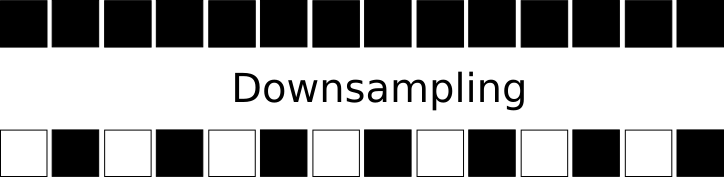
\includegraphics[width=0.4\linewidth]{images/downsampling}
				\label{fig:downsampling}
				\\Fonte: Elaborado pelo autor, 2023.
			\end{figure}
	
		\subsection{Caracterização dos processos de produção da voz humana}
			\par A fala possui três grandes áreas de estudo: A fisiológica, também conhecida como fonética articulatória, a acústica, referida como fonética acústica, e ainda, a perceptual, que cuida da percepção  da  fala \cite{kremer2014eficiencia}. Neste trabalho, o foco será apenas na questão acústica, pois não serão analisados aspectos da fisiologia relacionada à voz, mas sim os sinais sonoros propriamente ditos.
		
		\subsubsection{Sinais vozeados \textit{versus} não-vozeados}
			\par Quando da análise dos sinais de voz, consideram-se as partes vozeadas e não-vozeadas. Aquelas são produzidas com a ajuda da vibração quase periódica das pregas vocais, enquanto estas praticamente não contam com participação regrada da referida estrutura.
		
		\subsubsection{Frequência fundamental da voz}
			\par Também conhecida como $F_0$, é o componente periódico resultante da vibração das pregas vocais. Em termos de percepção, se pode interpretar $F_0$ como o tom da voz, isto é, a frequência de \textit{pitch} \cite{kremer2014eficiencia}. Vozes agudas tem uma frequência de \textit{pitch} alto, enquanto vozes mais graves tem baixa. A alteração da frequência (jitter) e/ou intensidade (shimmer) do \textit{pitch} durante a fala é definida como entonação,  porém, também pode indicar algum distúrbio ou doença relacionada ao trato vocal \cite{WERTZNER2005}.
			
			\par A frequência fundamental da voz é o número de vezes na qual uma forma de onda característica, que reflete a excitação pulmonar moldada pelas pregas vocais, se repete por unidade de tempo. Sendo assim, as medidas de $F_0$ geralmente são apresentadas em Hz \cite{freitas2013avaliaccao}.
			
			\par A medição de $F_0$ está sujeita a contaminações surgidas das variações naturais de \textit{pitch} típicas da voz humana \cite{freitas2013avaliaccao}. A importância de se medir $F_0$ corretamente vem do fato de que, além de carregar boa parte da informação da fala, ela é a base para construção das outras frequências que compõe os sinais de voz, que são múltiplas de $F_0$.
		
		\subsubsection{Formantes}
			\par O sinal de excitação que atravessa as pregas vocais é rico em harmônicas, isto é, frequências múltiplas da fundamental. Tais harmônicas podem ser atenuadas ou amplificadas, em função da estrutura dos tratos vocal e nasal de cada locutor. Particularmente, o primeiro formante ($F_1$), relaciona-se à  amplificação  sonora  na  cavidade  oral  posterior  e  à  posição  da  língua  no  plano  vertical;  o segundo  formante  ($F_2$)  à  cavidade  oral  anterior  e  à  posição  da  língua  no  plano  horizontal; o terceiro  formante  ($F_3$)  relaciona-se  às  cavidades  à  frente  e  atrás  do  ápice  da  língua e, finalmente,  o  quarto formante  ($F_4$) relaciona-se  ao  formato  da  laringe  e  da  faringe  na  mesma  altura  \cite{valencca2014analise}. Formantes caracterizam fortemente os locutores, pois cada indivíduo possui um formato de trato vocal e nasal. Assim, tais frequências, que podem ser capturadas com ferramentas diversas, a exemplo da Transformada \textit{Wavelet}, são de suma importância na área de verificação de locutores.
	
		\subsection{Escalas e energias dos sinais}
			\par A energia de um sinal digital $s[\cdot]$ com $M$ amostras é definida como
			
			\begin{equation}
				E = \sum\limits_{i=0}^{M-1}(s_i)^2 \qquad.   
			\end{equation}
			
			$E$ pode ainda sofrer normalizações e ter a sua mensuração restrita a uma parte específica do sinal sob análise. Possibilidades para tais restrições podem, por exemplo, envolver a escala BARK \cite{doi:10.1121-1.1908630} e MEL \cite{beranek1949acoustic} que serão utilizadas neste trabalho.
		\subsubsection{A escala BARK}
			\par BARK foi definida tendo em mente vários tipos de sinais acústicos. Essa escala corresponde ao conjunto de 25 bandas críticas da audição humana. Suas frequências-base de audiometria são, em Hz: \textbf{20, 100, 200, 300, 400, 510, 630, 770, 920, 1080, 1270, 1480, 1720, 2000, 2320, 2700, 3150, 3700, 4400, 5300, 6400, 7700, 9500, 12000, 15500}. Nessa escala,os sinais digitais no domínio temporal atravessam filtros passa-faixas \cite{bosi2002introduction} para os quais o início e o final da banda de passagem correspondem à frequências-base consecutivas resultando em um vetor de características com 24 coeficientes e, em seguida, as energias dos sinais filtrados são utilizadas como características descritivas de propriedades do sinal sob análise, como mostrado na Figura \ref{fig:barkfeaturevect}.
			\begin{figure}[h]
				\centering
				\caption{Cálculo de vetores de características com BARK}
				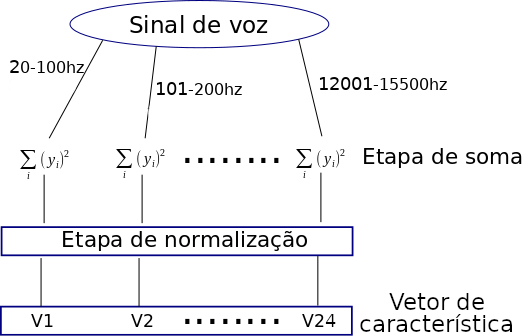
\includegraphics[width=0.6\linewidth]{images/barkFeatureVect}
				\label{fig:barkfeaturevect}
				\\Fonte: Elaborado pelo autor, 2023.
			\end{figure}
		\subsubsection{A escala MEL}
			\par Escala Mel, advinda do termo \textit{melody}, é uma adaptação da escala Bark para sinais de voz. Dentre as várias implementações de bandas críticas a escolhida foi a implementação que contém os valores em Hz: \textbf{20, 160, 394, 670, 1000, 1420, 1900, 2450, 3120, 4000, 5100, 6600, 9000, 14000}.
			
			\par A variante que será usada neste trabalho é conhecida como \textit{Mel-frequency cepstral coefficients}(MFCC) a qual inclui, além dos intervalos definidos, uma diminuição da correlação entre os componentes gerados via aplicação da Transformada Discreta Cosseno (DCT) \cite{salomon2007data} ou da Análise de Componentes Principais (PCA) \cite{jolliffe2006principal} seguida de duas derivações no vetor de características resultando em um total de 11 coeficientes. Nesse trabalho foi escolhida a DCT, no entanto, PCA poderia também ser escolhida sem prejuízos, o uso de uma ou outra depende da preferência do autor.
			
			\par Novamente, desconsiderando qualquer etapa intermediária que possa ser adicionada, as energias calculadas nos intervalos definidos na escala MEL podem, por si mesmas, constituir um vetor de características, como mostrado na Figura \ref{fig:barkfeaturevect}.
			
			\begin{figure}[h]
				\centering
				\caption{Cálculo de vetores de características com MEL}
				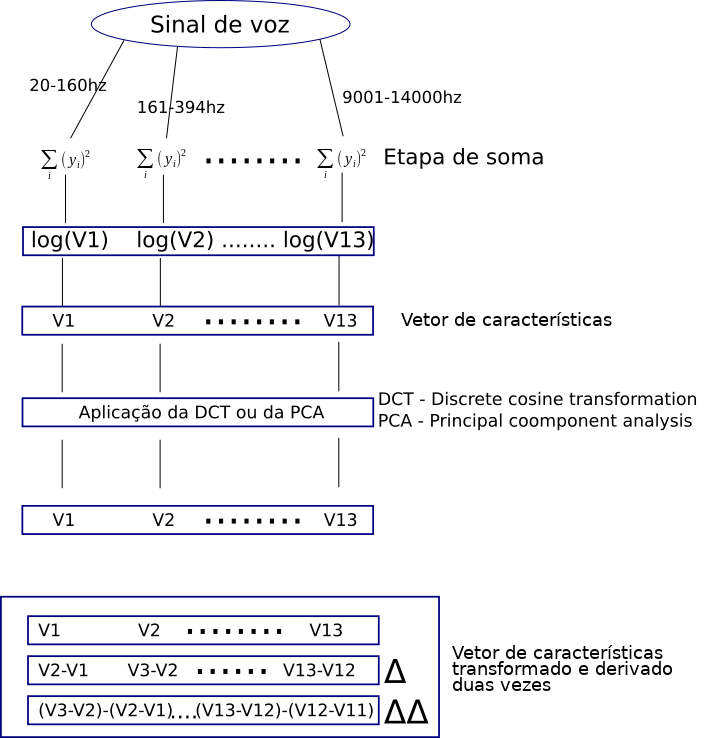
\includegraphics[width=0.8\linewidth]{images/melFeatureVect}
				\label{fig:melfeaturevect}
				\\Fonte: Elaborado pelo autor, 2023.
			\end{figure}
	
		\subsection{Filtros digitais \textit{wavelet}}
			\par Filtros digitais \textit{wavelet} têm sido utilizados com sucesso para suprir as deficiências de janelamento de sinal apresentadas pelas Transformadas de Fourier e de Fourier de Tempo Reduzido. \textit{Wavelets} contam com variadas funções-filtro e têm tamanho de janela variável, o que permite uma análise multirresolução \cite{Rod5254905}. Particularmente, as \textit{wavelets} proporcionam a análise do sinal de forma detalhada tanto no espectro de baixa frequência quanto no de alta contando com diferentes funções-base não periódicas diferentemente da tradicional transformada de Fourrier que utilizam somente as bases periódicas senoidal e cossenoidal.
			
			\par É importante observar que, quando se trata de Transformadas \textit{Wavelet}, seis elementos estão presentes: dois filtros de análise, dois filtros de síntese e as funções ortogonais \textit{scaling} e \textit{wavelet}. No tocante a sua aplicação, só a transformada direta, e não a inversa, será usada na construção dos vetores de características. Portanto, os filtros de síntese, a função \textit{scaling} e a função \textit{wavelet} não serão elementos abordados aqui: eles somente interessariam caso houvesse a necessidade da transformada inversa.
			
			\par No contexto dos filtros digitais baseados em \textit{wavelets}, o tamanho da janela recebe o nome de \textbf{suporte}. Janelas definem o tamanho do filtro que será aplicado ao sinal. Quando esse é pequeno (limitado), se diz que a janela tem \textbf{um suporte compacto} \cite{robi2003}.
			
			\par Se diz que uma \textit{wavelet} tem boa \textbf{resposta em frequência} quando, na aplicação da mesma para filtragem, não são causadas muitas pertubações indesejadas ao sinal, no domínio da frequência. Os filtros \textit{wavelet} de Daubechies \cite{daubechies1992ten} se destacam nesse quesito por serem \textit{maximamente planos} (\textit{maximally-flat}) \cite{butterworth1930} \cite{bianchi2007electronic} nos platôs de resposta em frequência como indicado na Figura \ref{fig:daubechies} ao contrário do que ocorre na Figura \ref{fig:nomaximallyflat}.
			
			\begin{figure}[h]
				\centering
				\caption{Platôs maximamente planos em um filtro digital: característica da família de Daubechies}
				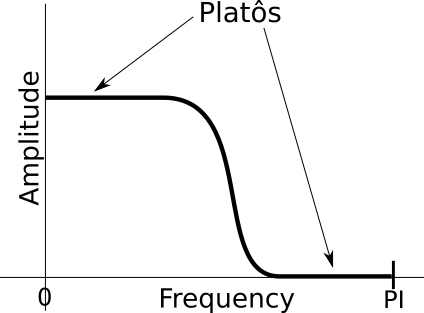
\includegraphics[width=0.3\linewidth]{images/daubechies}
				\label{fig:daubechies}
				\\Fonte: Elaborado pelo autor, 2023.
			\end{figure}
			
			\begin{figure}[h]
				\centering
				\caption{Platôs não maximamente planos de um filtro digital: características de outros filtros \textit{wavelet}, distintos da família de Daubechies}
				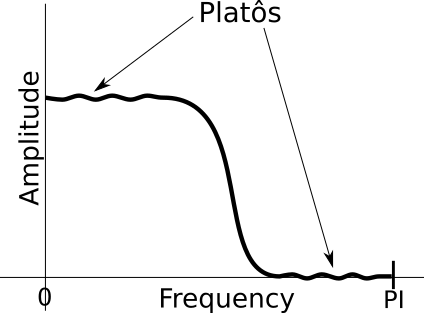
\includegraphics[width=0.3\linewidth]{images/noMaximallyFlat}
				\label{fig:nomaximallyflat}
				\\Fonte: Elaborado pelo autor, 2023.
			\end{figure}
			
			\par Além da resposta em frequência, na aplicação de um filtro digital \textit{wavelet} também é possível considerar a \textbf{resposta em fase}, que constitui um atraso ou adiantamento do sinal filtrado em relação ao sinal original, ambos no domínio temporal. Esse deslocamento pode ser \textbf{linear}, \textbf{quase linear} ou \textbf{não linear}: 
	
			\begin{itemize}
				\item na resposta em fase \textbf{linear}, há o mesmo deslocamento de fase para todos os componentes do sinal;
				\item quando a resposta em fase é \textbf{quase linear} existe uma pequena diferença no deslocamento dos diferentes componentes do sinal;
				\item finalmente, quando a resposta é \textbf{não linear}, acontece um deslocamento significativamente heterogêneo para as diferentes frequências que compõe o sinal.
			\end{itemize}
			
			\par Idealmente, é desejável que todo filtro apresente boa resposta em frequência e em fase linear. Características de fase e frequência de algumas famílias de filtros \textit{wavelet} constam na Tabela \ref{tab:waveletsProperties}.
			
			\begin{table}[h]
	\centering
	\caption{Algumas das \textit{wavelets} mais usadas e suas propriedades}
	\begin{tabular}{|c|p{75mm}|c|}
			\hline 
			\textbf{Wavelet} & \textbf{Resposta em frequência} & \textbf{Resposta em fase} \\ 
			\hline 
			Haar & Pobre &  Linear \\ 
			\hline 
			Daubechies & mais próxima da ideal à medida que o \newline  suporte aumenta; \textit{maximally-flat}  &  Não linear \\ 
			\hline 
			Symmlets & mais próxima da ideal à medida que o \newline  suporte aumenta; não \textit{maximally-flat}  & Quase linear \\ 
			\hline 
			Coiflets & mais próxima da ideal à medida que o \newline  suporte aumenta; não \textit{maximally-flat}  & Quase linear \\ 
			\hline 
	\end{tabular} 
	\label{tab:waveletsProperties}
	\\Fonte: Elaborado pelo autor, 2022.
\end{table}

	
		\subsubsection{O algoritmo de Mallat para a Transformada \textit{Wavelet}}
			\par Baseando-se no artigo \cite{7079589}, percebe-se que algoritmo de Mallat faz com que aplicação das \textit{wavelets} seja uma simples multiplicação de matrizes. O sinal que deve ser transformado se torna uma matriz linear vertical. Os filtros passa-baixa e passa-alta tornam-se, nessa ordem, linhas de uma matriz quadrada que será completada segundo regras que serão mostradas mais adiante. É importante que essa matriz quadrada tenha a mesma dimensão que o sinal a ser transformado.
			
			\par Interessantemente, para que seja possível a transformação \textit{wavelet}, basta ter disponível o vetor do filtro passa-baixas calculado a partir da \textit{mother wavelet}, que é a função geradora desse filtro, já que o passa-alta pode ser construído a partindo-se da ortogonalidade do primeiro.
			
			\par Determinar a ortogonal de um vetor significa construir um vetor, tal que, o produto escalar do vetor original com sua respectiva ortogonal seja nulo.
			
			\par Considerando $h[\cdot]$ como sendo o vetor do filtro passa-baixas e $g[\cdot]$ seu correspondente ortogonal, tem-se que $h[\cdot] \cdot g[\cdot] = 0 \qquad .$
			\par Portanto, se $h[\cdot]=[a, b, c, d]$ então seu ortogonal será $g[\cdot]=[d, -c, b, -a]$ pois:
			$$
			h[\cdot] \cdot g[\cdot]  =  [a, b, c, d] \cdot [d, -c, b, -a] = (a \cdot d) + (b \cdot (-c)) + (c \cdot b) + (d \cdot (-a)) = ad - ad + bc - bc = 0 \qquad.
			$$
	
			\par A título de exemplo, considera-se:
			\begin{itemize}
				\item o filtro passa baixa baseado na \textit{wavelet} Haar: $h[\cdot] = [\frac{1}{\sqrt{2}}, \frac{1}{\sqrt{2}}]$
				\item o seu respectivo vetor ortogonal: $g[\cdot] = [\frac{1}{\sqrt{2}}, \frac{-1}{\sqrt{2}}]$
				\item e também o seguinte sinal-exemplo de entrada: $s = \{1,2,3,4\}$
			\end{itemize}
			
			\par Se o tamanho do sinal a ser tratado é quatro e se pretende-se aplicar o filtro Haar, a seguinte matriz de coeficientes é construída:
			\begin{equation}
				\begin{pmatrix}
					\frac{1}{\sqrt{2}}, \frac{1}{\sqrt{2}}, 0, 0\\
					\frac{1}{\sqrt{2}}, \frac{-1}{\sqrt{2}}, 0, 0\\
					0, 0, \frac{1}{\sqrt{2}}, \frac{1}{\sqrt{2}}\\
					0, 0, \frac{1}{\sqrt{2}}, \frac{1}{\sqrt{2}}
					\label{eq:haarFilters}
				\end{pmatrix} 
			\end{equation}
		
			\par Tendo em vista que a dimensão do sinal sob análise é diferente da dimensão do filtro, basta completar cada uma das linhas da matriz de coeficientes com zeros. A matriz é montada de forma que ela seja ortogonal.
			
			\par Montada a matriz de filtros, segue-se com os cálculos da transformada:
			\begin{equation}
				\begin{pmatrix}
					\frac{1}{\sqrt{2}}, \frac{1}{\sqrt{2}}, 0, 0\\
					\frac{1}{\sqrt{2}}, \frac{-1}{\sqrt{2}}, 0, 0\\
					0, 0, \frac{1}{\sqrt{2}}, \frac{1}{\sqrt{2}}\\
					0, 0, \frac{1}{\sqrt{2}}, \frac{1}{\sqrt{2}}\\
				\end{pmatrix} 
				\cdot
				\begin{pmatrix}
					1\\
					2\\
					3\\
					4\\
				\end{pmatrix} 
				=
				\begin{pmatrix}
					\frac{3}{\sqrt{2}}\\
					\frac{-1}{\sqrt{2}}\\
					\frac{7}{\sqrt{2}}\\
					\frac{-1}{\sqrt{2}}
				\end{pmatrix}
				\label{eq:haarMultiplic}
			\end{equation}

			\par Realizada a multiplicação, é necessário montar o sinal filtrado. Isso é feito escolhendo, dentro do resultado, valores alternadamente de forma que o vetor resultante seja:
			
			\begin{equation}
				resultado = \Big[
				\frac{3}{\sqrt{2}},
				\frac{7}{\sqrt{2}},
				\frac{-1}{\sqrt{2}},
				\frac{-1}{\sqrt{2}}
				\Big]\qquad.
				\label{eq:haarResult}
			\end{equation}
			
			\par Percebe-se que, na transformação descrita nas Equações \ref{eq:haarFilters}, \ref{eq:haarMultiplic} e \ref{eq:haarResult}, a \textbf{aplicação dos filtros sobre o vetor de entrada ocorreu apenas uma vez}. Sendo assim, se diz que o sinal recebeu uma \textbf{transformação de nível 1}. A cada transformação, há uma separação do sinal em dois componentes: o de baixa e o de alta frequência.
	
			\par Embora haja um limite, que será mencionado adiante, é possível aplicar mais de um nível de decomposição ao sinal. Para que se possa fazer isso, a Transformada \textit{Wavelet} nível 2 deve considerar apenas a parte de baixas frequências da primeira transformada; a transformada de nível 3 deve considerar apenas a parte de baixas frequências da transformada nível 2, e assim consecutivamente.
			
			\par Nos exemplos numéricos mostrados nas Tabelas \ref{tab:regularWaveletExample}, \ref{tab:packetWaveletExampleLF} e \ref{tab:packetWaveletExampleHF}, usou-se um filtro normalizado cujos coeficientes são $\{\dfrac{1}{2},-\dfrac{1}{2}\}$. Os dados destacados em \textbf{verde} correspondem ao \textbf{vetor original} que será tratado. Cada uma das linhas são os resultados das transformações nos níveis 1, 2, 3 e 4, respectivamente. As partes em \textbf{azul} correspondem à porção de \textbf{baixas frequências}, enquanto que as partes em \textbf{amarelo} correspondem às porções de \textbf{altas frequências}.
			
			\par Percebe-se que na Tabela \ref{tab:regularWaveletExample}, a partir da transformação nível 2, apenas as partes de baixa frequência são modificadas. Isso implica que, no momento da implementação do algoritmo de Mallat \textbf{para níveis maiores que 1}, a abordagem será \textbf{recursiva}. Em outras palavras, a partir do nível 1 se deve aplicar Mallat apenas às porções de baixas-frequências geradas pela transformação anterior.
	
			\begin{table}[h]
	\fontsize{9}{\baselineskip} \selectfont
	\newcommand{\mc}[3]{\multicolumn{#1}{#2}{#3}}
	\definecolor{tcA}{rgb}{0.65098,0.65098,0.65098}
	\definecolor{tcD}{rgb}{1,0.94902,0}
	\definecolor{tcC}{rgb}{0,0.5,1}
	\definecolor{tcB}{rgb}{0.447059,0.74902,0.266667}
	\begin{center}
		\caption[Exemplo numérico da transformação \textit{wavelet}]{Exemplo numérico da transformação \textit{wavelet} aplicada a um vetor. Tabela completa no \autoref{sec:aplicaWavelet}.}
		\begin{tabular}{c|ccccccccccccccc|c}
			% use packages: color,colortbl
			\mc{1}{>{\columncolor{tcA}}c|}{\textbf{Sinal}} & \mc{1}{>{\columncolor{tcB}}c}{\textbf{32}} & \mc{1}{>{\columncolor{tcB}}c}{\textbf{10}} & \mc{1}{>{\columncolor{tcB}}c}{\textbf{20}} & \mc{1}{>{\columncolor{tcB}}c}{\textbf{38}} & \mc{1}{>{\columncolor{tcB}}c}{\textbf{37}} & \mc{1}{>{\columncolor{tcB}}c}{\textbf{28}} & \mc{1}{>{\columncolor{tcB}}c}{\textbf{38}} & \mc{1}{>{\columncolor{tcB}}c}{\textbf{34}} & \mc{1}{>{\columncolor{tcB}}c}{\textbf{18}} & \mc{1}{>{\columncolor{tcB}}c}{\textbf{24}} & \mc{1}{>{\columncolor{tcB}}c}{\textbf{24}} & \mc{1}{>{\columncolor{tcB}}c}{\textbf{9}} & \mc{1}{>{\columncolor{tcB}}c}{\textbf{23}} & \mc{1}{>{\columncolor{tcB}}c}{\textbf{24}} & \mc{1}{>{\columncolor{tcB}}c}{\textbf{28}} & \mc{1}{>{\columncolor{tcB}}c}{\textbf{34}}\\
			\hline
			
			\mc{1}{>{\columncolor{tcA}}c|}{Nível 01} & \mc{1}{>{\columncolor{tcC}}c}{21} & \mc{1}{>{\columncolor{tcC}}c}{29} & \mc{1}{>{\columncolor{tcC}}c}{32,5} & \mc{1}{>{\columncolor{tcC}}c}{36} & \mc{1}{>{\columncolor{tcC}}c}{21} & \mc{1}{>{\columncolor{tcC}}c}{16,5} & \mc{1}{>{\columncolor{tcC}}c}{23,5} & \mc{1}{>{\columncolor{tcC}}c}{31} & \mc{1}{>{\columncolor{tcD}}c}{11} & \mc{1}{>{\columncolor{tcD}}c}{-9} & \mc{1}{>{\columncolor{tcD}}c}{4,5} & \mc{1}{>{\columncolor{tcD}}c}{2} & \mc{1}{>{\columncolor{tcD}}c}{-3} & \mc{1}{>{\columncolor{tcD}}c}{7,5} & \mc{1}{>{\columncolor{tcD}}c}{-0,5} & \mc{1}{>{\columncolor{tcD}}c}{-3}\\
			\hline
			
			\mc{1}{>{\columncolor{tcA}}c|}{Nível 02} & \mc{1}{>{\columncolor{tcC}}c}{25} & \mc{1}{>{\columncolor{tcC}}c}{34,25} & \mc{1}{>{\columncolor{tcC}}c}{18,75} & \mc{1}{>{\columncolor{tcC}}c}{27,25} & \mc{1}{>{\columncolor{tcD}}c}{-4} & \mc{1}{>{\columncolor{tcD}}c}{-1,75} & \mc{1}{>{\columncolor{tcD}}c}{2,25} & \mc{1}{>{\columncolor{tcD}}c}{-3,75} & \mc{1}{>{\columncolor{tcD}}c}{11} & \mc{1}{>{\columncolor{tcD}}c}{-9} & \mc{1}{>{\columncolor{tcD}}c}{4,5} & \mc{1}{>{\columncolor{tcD}}c}{2} & \mc{1}{>{\columncolor{tcD}}c}{-3} & \mc{1}{>{\columncolor{tcD}}c}{7,5} & \mc{1}{>{\columncolor{tcD}}c}{-0,5} & \mc{1}{>{\columncolor{tcD}}c}{-3}\\
			\hline
			
			\mc{1}{>{\columncolor{tcA}}c|}{Nível 03} & \mc{1}{>{\columncolor{tcC}}c}{29,62} & \mc{1}{>{\columncolor{tcC}}c}{23} & \mc{1}{>{\columncolor{tcD}}c}{-4,625} & \mc{1}{>{\columncolor{tcD}}c}{-4,25} & \mc{1}{>{\columncolor{tcD}}c}{-4} & \mc{1}{>{\columncolor{tcD}}c}{-1,75} & \mc{1}{>{\columncolor{tcD}}c}{2,25} & \mc{1}{>{\columncolor{tcD}}c}{-3,75} & \mc{1}{>{\columncolor{tcD}}c}{11} & \mc{1}{>{\columncolor{tcD}}c}{-9} & \mc{1}{>{\columncolor{tcD}}c}{4,5} & \mc{1}{>{\columncolor{tcD}}c}{2} & \mc{1}{>{\columncolor{tcD}}c}{-3} & \mc{1}{>{\columncolor{tcD}}c}{7,5} & \mc{1}{>{\columncolor{tcD}}c}{-0,5} & \mc{1}{>{\columncolor{tcD}}c}{-3}\\
			\hline
			
			\mc{1}{>{\columncolor{tcA}}c|}{Nível 04} & \mc{1}{>{\columncolor{tcC}}c}{26,3125} & \mc{1}{>{\columncolor{tcD}}c}{3,3125} & \mc{1}{>{\columncolor{tcD}}c}{-4,625} & \mc{1}{>{\columncolor{tcD}}c}{-4,25} & \mc{1}{>{\columncolor{tcD}}c}{-4} & \mc{1}{>{\columncolor{tcD}}c}{-1,75} & \mc{1}{>{\columncolor{tcD}}c}{2,25} & \mc{1}{>{\columncolor{tcD}}c}{-3,75} & \mc{1}{>{\columncolor{tcD}}c}{11} & \mc{1}{>{\columncolor{tcD}}c}{-9} & \mc{1}{>{\columncolor{tcD}}c}{4,5} & \mc{1}{>{\columncolor{tcD}}c}{2} & \mc{1}{>{\columncolor{tcD}}c}{-3} & \mc{1}{>{\columncolor{tcD}}c}{7,5} & \mc{1}{>{\columncolor{tcD}}c}{-0,5} & \mc{1}{>{\columncolor{tcD}}c}{-3}
		\end{tabular}
		\label{tab:regularWaveletExample}
		\fontsize{12}{\baselineskip} \selectfont
		\\Fonte: Elaborado pelo autor, 2022.
	\end{center}
\end{table}
	
		\subsubsection{O algoritmo de Mallat e a Transformada \textit{Wavelet-Packet}}
			\par Na Transformada \textit{Wavelet-Packet}, os filtros aplicados são os mesmos da Transformada \textit{Wavelet} e o procedimento recursivo de cálculo também é o mesmo, no entanto, realizada a transformação de nível 1, a transformada de nível 2 deve ser aplicada aos componentes de baixa e de alta frequência. Sendo assim a Transformada \textit{Wavelet-Packet} obtém um nível de detalhes em todo o espectro de frequência, maior do que uma transformação regular. 
			
			\par Os exemplos mostrados nas Tabelas \ref{tab:packetWaveletExampleLF} e \ref{tab:packetWaveletExampleHF} permitem perceber como se dão as transformações na porção de \textbf{baixa} e de \textbf{alta} frequências, respectivamente, após a transformação \textit{wavelet-packet} de nível 1, 2, 3 e 4.
			
			\par Devido ao \textit{downsampling} aplicado às porções de alta frequência, essas partes acabam por ficar ``espelhadas'' no espectro \cite{Jensen_2001}, ou seja, suas sequências ficam invertidas. Para resolver esse problema e preservar a ordem das sub-bandas no sinal transformado, os filtros são aplicados em ordem inversa nas porções de alta frequência. Isso altera como o algoritmo de Mallat deve ser implementado para a Transformada \textit{Wavelet-Packet}, já que dessa vez é preciso se atentar a ordem da aplicação dos filtros passa-alta e passa-baixa.
	
			\begin{table}[h]
	\newcommand{\mc}[3]{\multicolumn{#1}{#2}{#3}}
	\definecolor{tcA}{rgb}{0.65098,0.65098,0.65098}
	\definecolor{tcD}{rgb}{1,0.94902,0}
	\definecolor{tcC}{rgb}{0,0.5,1}
	\definecolor{tcB}{rgb}{0.447059,0.74902,0.266667}
	\begin{center}
		\caption{Exemplo numérico de \textit{wavelet-packet} Haar aplicada ao vetor da Tabela \ref{tab:regularWaveletExample} (porção das baixas frequências)}
		\begin{tabular}{l|llllllll|}
			% use packages: color,colortbl
			\mc{1}{>{\columncolor{tcA}}l|}{\textbf{Sinal}} & \mc{1}{>{\columncolor{tcB}}l}{\textbf{32}} & \mc{1}{>{\columncolor{tcB}}l}{\textbf{10}} & \mc{1}{>{\columncolor{tcB}}l}{\textbf{20}} & \mc{1}{>{\columncolor{tcB}}l}{\textbf{38}} & \mc{1}{>{\columncolor{tcB}}l}{\textbf{37}} & \mc{1}{>{\columncolor{tcB}}l}{\textbf{28}} & \mc{1}{>{\columncolor{tcB}}l}{\textbf{38}} & \mc{1}{>{\columncolor{tcB}}l|}{\textbf{34}}\\
			\hline
			
			\mc{1}{>{\columncolor{tcA}}l|}{Nivel 01} & \mc{1}{>{\columncolor{tcC}}l}{21} & \mc{1}{>{\columncolor{tcC}}l}{29} & \mc{1}{>{\columncolor{tcC}}l}{32,5} & \mc{1}{>{\columncolor{tcC}}l}{36} & \mc{1}{>{\columncolor{tcC}}l}{21} & \mc{1}{>{\columncolor{tcC}}l}{16,5} & \mc{1}{>{\columncolor{tcC}}l}{23,5} & \mc{1}{>{\columncolor{tcC}}l|}{31}\\
			\hline
			
			\mc{1}{>{\columncolor{tcA}}l|}{Nivel 02} & \mc{1}{>{\columncolor{tcC}}l}{25} & \mc{1}{>{\columncolor{tcC}}l}{34,25} & \mc{1}{>{\columncolor{tcC}}l}{18,75} & \mc{1}{>{\columncolor{tcC}}l|}{27,25} & \mc{1}{>{\columncolor{tcD}}l}{-4} & \mc{1}{>{\columncolor{tcD}}l}{-1,75} & \mc{1}{>{\columncolor{tcD}}l}{2,25} & \mc{1}{>{\columncolor{tcD}}l|}{-3,75}\\
			\hline
			
			\mc{1}{>{\columncolor{tcA}}l|}{Nivel 03} & \mc{1}{>{\columncolor{tcC}}l}{29,62} & \mc{1}{>{\columncolor{tcC}}l|}{23} & \mc{1}{>{\columncolor{tcD}}l}{-4,625} & \mc{1}{>{\columncolor{tcD}}l|}{-4,25} & \mc{1}{>{\columncolor{tcD}}l}{-1,125} & \mc{1}{>{\columncolor{tcD}}l|}{3} & \mc{1}{>{\columncolor{tcC}}l}{-2,875} & \mc{1}{>{\columncolor{tcC}}l|}{-0,75}\\
			\hline
			
			\mc{1}{>{\columncolor{tcA}}l|}{Nivel 04} & \mc{1}{>{\columncolor{tcC}}l|}{26,3125} & \mc{1}{>{\columncolor{tcD}}l|}{3,3125} & \mc{1}{>{\columncolor{tcD}}l|}{-0,1875} & \mc{1}{>{\columncolor{tcC}}l|}{-4,4375} & \mc{1}{>{\columncolor{tcC}}l|}{0,9375} & \mc{1}{>{\columncolor{tcD}}l|}{-2,0625} & \mc{1}{>{\columncolor{tcD}}l|}{-1,0625} & \mc{1}{>{\columncolor{tcC}}l|}{-1,8125}\\
		\end{tabular}
		\label{tab:packetWaveletExampleLF}
		\\Fonte: Elaborado pelo autor, 2023.
	\end{center}
\end{table}

\begin{table}[h]
	\newcommand{\mc}[3]{\multicolumn{#1}{#2}{#3}}
	\definecolor{tcA}{rgb}{0.65098,0.65098,0.65098}
	\definecolor{tcC}{rgb}{1,0.94902,0}
	\definecolor{tcD}{rgb}{0,0.5,1}
	\definecolor{tcB}{rgb}{0.447059,0.74902,0.266667}
	\begin{center}
		\caption{Exemplo numérico de \textit{wavelet-packet} Haar aplicada ao vetor da Tabela \ref{tab:regularWaveletExample} (porção das altas frequências)}
		\begin{tabular}{c|cccccccc}
			% use packages: color,colortbl
			\mc{1}{>{\columncolor{tcA}}c|}{\textbf{Sinal}} & \mc{1}{>{\columncolor{tcB}}c}{\textbf{18}} & \mc{1}{>{\columncolor{tcB}}c}{\textbf{24}} & \mc{1}{>{\columncolor{tcB}}c}{\textbf{24}} & \mc{1}{>{\columncolor{tcB}}c}{\textbf{9}} & \mc{1}{>{\columncolor{tcB}}c}{\textbf{23}} & \mc{1}{>{\columncolor{tcB}}c}{\textbf{24}} & \mc{1}{>{\columncolor{tcB}}c}{\textbf{28}} & \mc{1}{>{\columncolor{tcB}}c|}{\textbf{34}}\\\hline
			\mc{1}{>{\columncolor{tcA}}c|}{Nivel 01} & \mc{1}{>{\columncolor{tcC}}c}{11} & \mc{1}{>{\columncolor{tcC}}c}{-9} & \mc{1}{>{\columncolor{tcC}}c}{4,5} & \mc{1}{>{\columncolor{tcC}}c}{2} & \mc{1}{>{\columncolor{tcC}}c}{-3} & \mc{1}{>{\columncolor{tcC}}c}{7,5} & \mc{1}{>{\columncolor{tcC}}c}{-0,5} & \mc{1}{>{\columncolor{tcC}}c|}{-3}\\\hline
			\mc{1}{>{\columncolor{tcA}}c|}{Nivel 02} & \mc{1}{>{\columncolor{tcC}}c}{10} & \mc{1}{>{\columncolor{tcC}}c|}{1,25} & \mc{1}{>{\columncolor{tcC}}c}{-5,25} & \mc{1}{>{\columncolor{tcC}}c|}{1,25} & \mc{1}{>{\columncolor{tcD}}c}{1} & \mc{1}{>{\columncolor{tcD}}c|}{3,25} & \mc{1}{>{\columncolor{tcD}}c}{2,25} & \mc{1}{>{\columncolor{tcD}}c|}{-1,75}\\\hline
			\mc{1}{>{\columncolor{tcA}}c|}{Nivel 03} & \mc{1}{>{\columncolor{tcD}}c|}{5,625} & \mc{1}{>{\columncolor{tcD}}c|}{-2} & \mc{1}{>{\columncolor{tcC}}c|}{4,375} & \mc{1}{>{\columncolor{tcC}}c|}{-3,25} & \mc{1}{>{\columncolor{tcC}}c|}{-1,125} & \mc{1}{>{\columncolor{tcC}}c|}{2} & \mc{1}{>{\columncolor{tcD}}c|}{2,125} & \mc{1}{>{\columncolor{tcD}}c|}{0,25}\\\hline
			
			\mc{1}{>{\columncolor{tcA}}c|}{Nivel 04} & \mc{1}{>{\columncolor{tcD}}c|}{1,8125} & \mc{1}{>{\columncolor{tcC}}c|}{3,8125} & \mc{1}{>{\columncolor{tcC}}c|}{3,8125} & \mc{1}{>{\columncolor{tcD}}c|}{0,5625} & \mc{1}{>{\columncolor{tcD}}c|}{0,4375} & \mc{1}{>{\columncolor{tcC}}c|}{-1,5625} & \mc{1}{>{\columncolor{tcC}}c|}{0,9375} & \mc{1}{>{\columncolor{tcD}}c|}{1,1875}\\
		\end{tabular}
		\label{tab:packetWaveletExampleHF}
		\\Fonte: Elaborado pelo autor, 2023.
	\end{center}
\end{table}
	
		\subsection{Engenharia Paraconsistente de características}
			\par Nos processos de classificação, frequentemente surge a questão: ``Os vetores de características criados proporcionam uma boa separação de classes?''. A Engenharia Paraconsistente de Características, recém publicada \cite{8588433}, que usa a paraconsistência \cite{da1998elementos},  \cite{COSTA2000} é, em meio a outras técnicas, uma ferramenta que pode ser usada para responder essa questão.
			
			\par O processo inicia-se após a aquisição dos vetores de características para cada classe $C_n$. Se o número de classes presentes for, por exemplo, quatro então estas poderão ser representadas por $C_1, C_2, C_3, C_4$.
			\par Em seguida é necessário o cálculo de duas grandezas:
			
			\begin{itemize}
				\item a menor similaridade intraclasse, $\alpha$.
				\item a razão de sobreposição interclasse, $\beta$.
			\end{itemize}
	
			\par $\alpha$ indica o quanto de similaridade os dados têm entre si, dentro de uma mesma classe, enquanto $\beta$ é a razão de sobreposição entre diferentes classes. Idealmente, $\alpha$ deve ser maximizada e $\beta$ minimizada para que classificadores extremamente modestos apresentem uma acurácia interessante.
			
			\par Particularmente, para calcular $\alpha$ e $\beta$, é necessária a normalização dos vetores de características de forma que todos os seus componentes estejam no intervalo entre $0$ e $1$. Em seguida, a obtenção de $\alpha$ se dá selecionando-se os maiores e os menores valores de cada uma das posições de todos os vetores de características para cada classe, gerando assim um vetor para os valores maiores e outro para os menores.
			
			\par O \textbf{vetor de similaridade da classe}$(svC_n)$ é obtido fazendo-se a diferença item-a-item dos maiores em relação aos menores. Finalmente, e para cada classe, é obtida a média dos valores para cada vetor de similaridade, sendo que $\alpha$ é o menor valor dentre essas médias. A Figura \ref{fig:calculoalpha} contém uma ilustração do processo.
	
			\begin{figure}[h]
				\centering
				\caption{Cálculo do coeficiente $\alpha$.}
				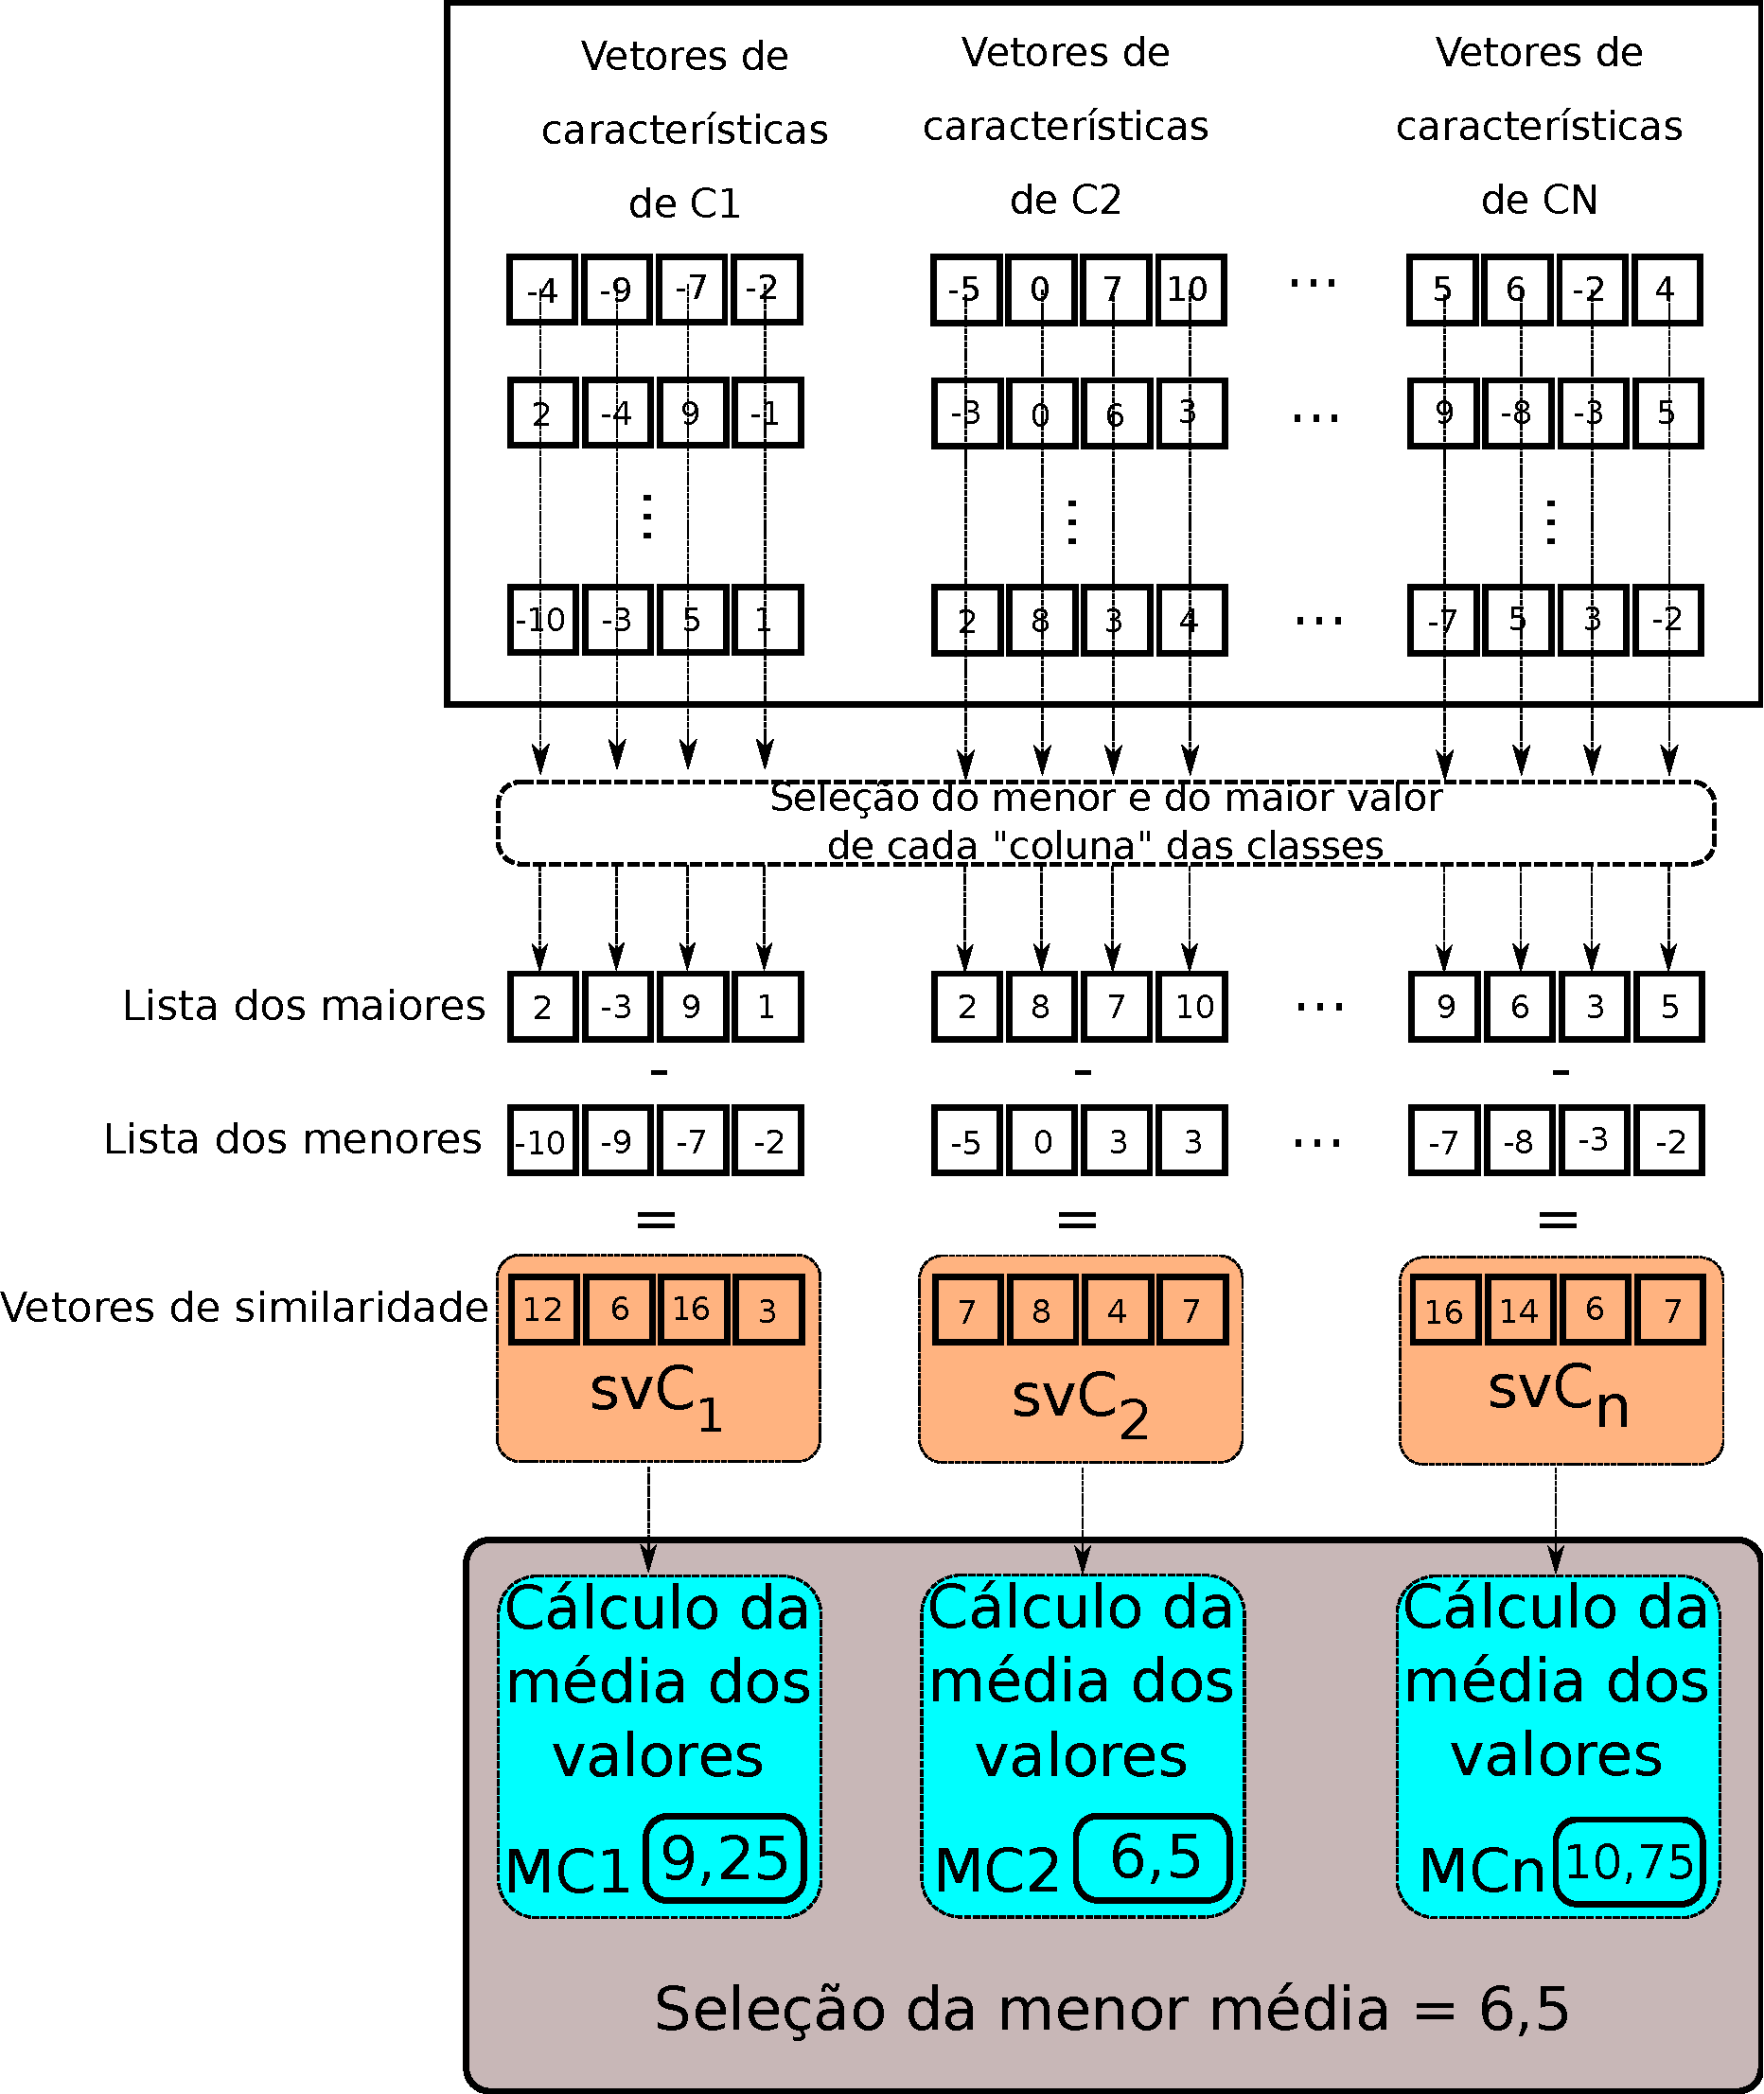
\includegraphics[width=0.5\linewidth]{images/calculoAlpha.pdf}
				\label{fig:calculoalpha}
				\\Fonte: Adaptado de \cite{8588433}.
			\end{figure}
			
			\par A obtenção de $\beta$, assim como ilustrado na Figura \ref{fig:betacalculation}, também se dá selecionando os maiores e os menores valores de cada uma das posições de todos os vetores de características de cada classe, gerando assim um vetor para os valores maiores e outro para os menores.
			
			\par Na sequência, realiza-se o cálculo de $R$ cujo valor é a quantidade de vezes que um valor do vetor de características de uma classe se encontra entre os valores maiores e menores de outra classe.
			
			\par Seja:
			\begin{itemize}
				\item N a quantidades de classes;
				\item X a quantidade de vetores de características por classe;
				\item T o tamanho do vetor de características.
			\end{itemize}
			
			\par Então, $F$, que é o número máximo de sobreposições possíveis entre classes, é dado por:
			\begin{equation}
				F=N.(N-1).X.T \qquad.
			\end{equation}
			\par Finalmente, $\beta$ é calculado da seguinte forma:
			\begin{equation}
				\beta=\dfrac{R}{F} \qquad.
			\end{equation}
	
			\par Neste ponto, é importante notar que $\alpha=1$ sugere fortemente que os vetores de características de cada classe são similares e representam suas respectivas classes precisamente. Complementarmente, $\beta=0$ sugere os vetores de características de classes diferentes não se sobrepõe \cite{8588433}.
			
			\begin{figure}[h]
				\centering
				\caption{Cálculo de $\beta$: Os itens destacados em azul e rosa são aqueles pertencentes a classe C1 e CN que se sobrepõe, em verde, a sobreposição é entre C1 e C2. Para cada sobreposição verificada soma-se 1 ao valor $R$. Essa comparação é feita para todos os vetores de características de cada uma das classes.}
				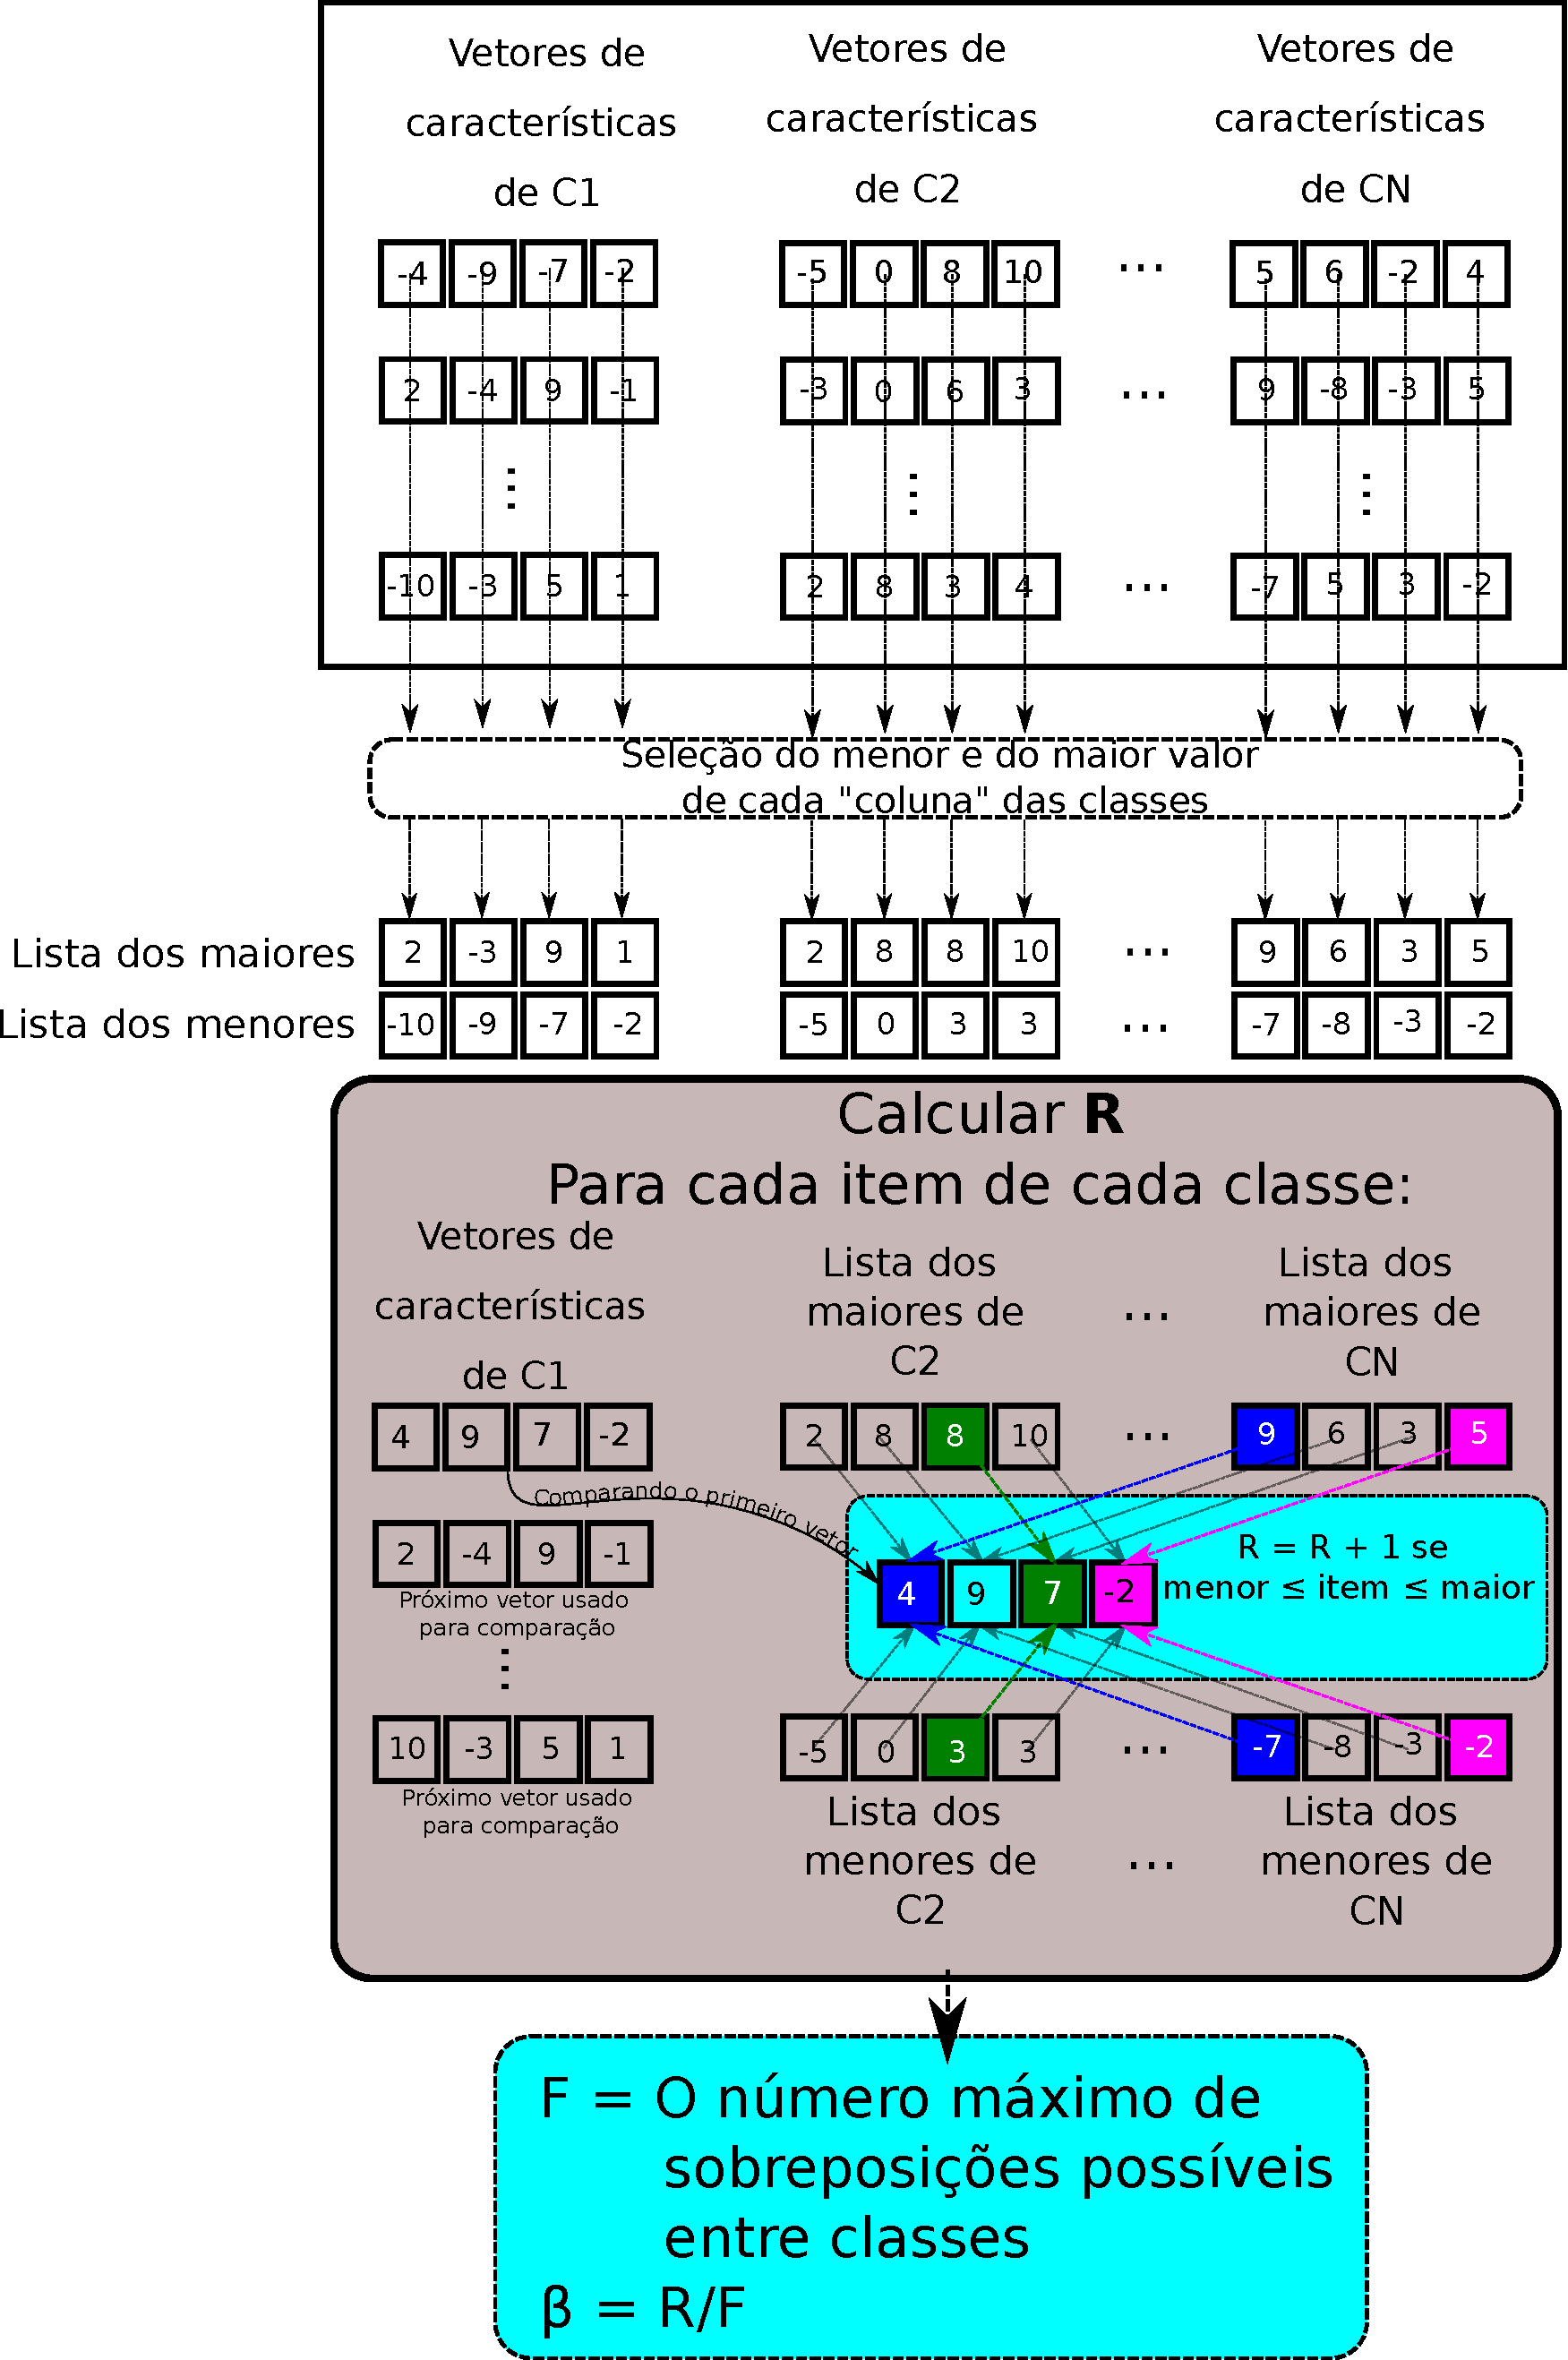
\includegraphics[width=0.5\linewidth]{images/betaCalculation.pdf}
				\label{fig:betacalculation}
				\\Fonte: Adaptado de \cite{8588433}.
			\end{figure}
			
			\par Considerando-se o plano paraconsistente \cite{8588433}, temos: 
			
			\begin{itemize}
				\item Verdade $\rightarrow$ fé total ($\alpha = 1$) e nenhum descrédito ($\beta = 0$)
				\item Ambiguidade $\rightarrow$ fé total ($\alpha = 1$) e descrédito total ($\beta = 1$)
				\item Falsidade $\rightarrow$ fé nula ($\alpha = 0$) e descrédito total ($\beta = 1$)
				\item Indefinição $\rightarrow$ fé nula ($\alpha = 0$) e nenhum descrédito ($\beta = 0$) \qquad.
			\end{itemize}
	
			\par No entanto, raramente $\alpha$ e $\beta$ terão valores inteiros como os mostrados na listagem acima: Na maioria das ocasiões, $0 \leqslant \alpha \leqslant 1$ e $0 \leqslant \beta \leqslant 1$. Por isso, se torna necessário o cálculo do \textbf{grau de certeza}, isto é, $G_1$, e do \textbf{grau de contradição}, isto é, $G_2$, conforme segue:
			\begin{equation}
				G_1=\alpha-\beta  \qquad,
			\end{equation}
			\begin{equation}
				G_2=\alpha+\beta-1 \qquad,
			\end{equation}
			onde: $-1 \leqslant G_1$ e  $1 \geqslant G_2$.
			
			\par Os valores de $G_1$ e $G_2$, em conjunto, definem os graus entre verdade ($G_1=1$) e falsidade ($G_1=-1$) e também os graus entre indefinição ($G_2=-1$) e ambiguidade ($G_2=1$). Novamente, raramente tais valores inteiros serão alcançados já que $G_1$ e $G_2$ dependem de $\alpha$ e $\beta$.
	
			\par O Plano Paraconsistente, para fins de visualização e maior rapidez na avaliação dos resultados, encontra-se ilustrado na Figura \ref{fig:paraconsistentplane} e tem quatro arestas precisamente definidas:
			\begin{itemize}
				\item (-1,0) $\rightarrow$ falsidade;
				\item (1,0) $\rightarrow$ verdade;
				\item (0,-1) $\rightarrow$ indefinição;
				\item (0,1) $\rightarrow$ ambiguidade.
			\end{itemize}
			\par A propósito de ilustração na Figura \ref{fig:paraconsistentplane}, é possível ver um pequeno círculo indicando os graus dos quatro casos listados.
			
			\par Para se ter ideia em que área exatamente se encontram as classes avaliadas, as distâncias $(D)$ do ponto $P=(G_1,G_2)$ até o limites supracitados podem ser computadas. Tais cálculos podem ser feitos da seguinte forma:
	
			\begin{equation}
				D_{-1,0}=\sqrt{(G_1+1)^2+(G_2)^2}\qquad,
			\end{equation}
			\begin{equation}
				D_{1,0}=\sqrt{(G_1-1)^2+(G_2)^2}\qquad,
			\end{equation}
			\begin{equation}
				D_{0,-1}=\sqrt{(G_1)^2+(G_2+1)^2}\qquad,		
			\end{equation}
			\begin{equation}
				D_{0,1}=\sqrt{(G_1)^2+(G_2-1)^2}\qquad.
			\end{equation}		
			
			\begin{figure}[H]
				\centering
				\caption{O plano paraconsistente: O pequeno círculo indica os graus de falsidade(-1,0), verdade(1,0), indefinição(0,-1) e ambiguidade(0,1)}
				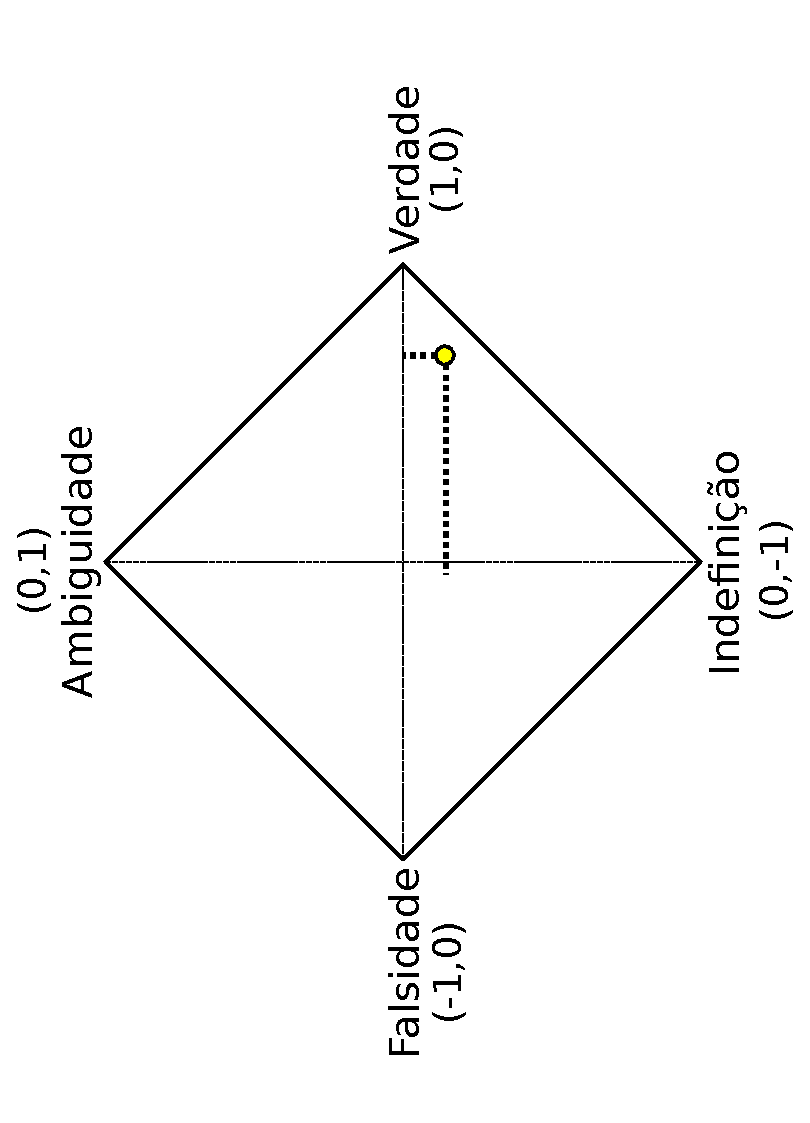
\includegraphics[angle=-90, width=0.69\linewidth]{images/paraconsistentPlane.pdf}
				\label{fig:paraconsistentplane}
				\\Fonte: Adaptado de \cite{8588433}.
			\end{figure}
			\par Na prática, ou seja, para fins de classificação, geralmente considera-se a distância em relação ao ponto \textit{``(1,0) $\rightarrow$ Verdade''}, que é o ponto ótimo: quanto mais próximo o ponto $(G_1,G_2)$ estiver de $(1,0)$, mais as os vetores de características das diferentes classes estão naturalmente separados. Isso implica, dentro da limitação de cada algoritmo, em resultados melhores sejam quais forem os classificadores usados.
	
	\subsection{Interfaces Humano-Máquina e EEG}
		
		\par Entre os métodos de Interface Cérebro-Computador (BCI), o Eletroencefalograma (EEG) se destaca como o sistema mais econômico e simples de implementar. No entanto, ele possui algumas peculiaridades, como alta sensibilidade a interferência eletromagnética e dificuldade em capturar o sinal devido a posicionamentos subótimos dos eletrodos no couro cabeludo. Portanto, um dos aspectos fundamentais que qualquer sistema de processamento de EEG deve ter é a tolerância ao ruído \cite{JALALYBIDGOLY2020101788}.
		
		\par Os eletrodos \textit{úmidos} são colocados usando gel condutivo e são menos propensos a artefatos provocados por movimentos, que são interferências eletromagnéticas causadas, por exemplo, ao piscar dos olhos. Os eletrodos \textit{secos} não precisam do gel, mas são mais sensíveis a tais artefatos.
		
		\par O EEG registra as atividades elétricas do cérebro, geralmente colocando eletrodos ao longo da superfície do couro cabeludo. Essas atividades elétricas resultam de fluxos de corrente iônica induzidos pela ativação sináptica sincronizada dos neurônios do cérebro. Elas se manifestam como flutuações de voltagem rítmicas com amplitude variando de 5 a 100$\mu V$ e frequência entre 0,5 e 40 Hz \cite{JALALYBIDGOLY2020101788}. As bandas de frequência operacionais no cérebro são as seguintes \cite{sanei2021eeg}:
		
		\begin{itemize}
			\item \textbf{Delta (1–4Hz)}: A onda mais lenta e geralmente a de maior amplitude. A banda Delta é observada em bebês e durante o sono profundo em adultos.
			
			\item \textbf{Theta (4–8Hz)}: Observada em crianças, adultos sonolentos e durante a recordação de memórias. A amplitude da onda Theta é tipicamente inferior a 100$\mu V$.
			
			\item \textbf{Alpha (8–12Hz)}: Geralmente a banda de frequência dominante, aparecendo durante a consciência relaxada ou quando os olhos estão fechados. A atenção focada ou a relaxamento com os olhos abertos reduzem a amplitude da banda Alpha. Essas ondas tem amplitudes normalmente inferiores a 50 $\mu V$.
			
			\item \textbf{Beta (12–25Hz)}: Associada ao pensamento, concentração ativa e atenção focada. A amplitude da onda Beta é normalmente inferior a 30 $\mu V$.
			
			\item \textbf{Gamma (acima de 25Hz)}: Observada durante o processamento sensorial múltiplo. Os padrões Gamma têm a menor amplitude.
			
		\end{itemize}
		
		\par De acordo com \cite{JALALYBIDGOLY2020101788}, para a maioria das tarefas realizadas pelo cérebro, existem regiões associadas a elas, conforme visto na Tabela \ref{tb:brainRegions}.
		
		\subsection{Sistema 10-20 e as áreas do cérebro}
		\begin{table}[H]
			\begin{center}
				\caption{Tarefas cerebrais e suas regiões correspondentes. Veja a Figura \ref{fig:1020standardandlobes} para mais informações.}
				\begin{tabular}{|c|c|p{0.4\textwidth}|}
					\hline
					Região & Canais & Tarefas\\
					\hline
					Lobo frontal & Fp1, Fp2, Fpz, Pz, F3, F7, F4, F8 & Memória, concentração, emoções.\\
					\hline
					Lobo parietal & P3, P4, Pz & Resolução de problemas, atenção, sentido do tato. \\
					\hline
					Lobo temporal & T3, T5, T4, T6 & Memória, reconhecimento de faces, audição, palavras e percepção social. \\
					\hline
					Lobo occipital & O1, O2, Oz & Leitura, visão.\\
					\hline
					Cerebelo && Controle motor, equilíbrio. \\
					\hline
					Córtex senso-motor & C3, C4, Cz& Atenção, processamento mental, controle motor fino, integração sensorial. \\
					\hline
				\end{tabular}
				\label{tb:brainRegions}
			\end{center}
		\end{table}
		
		\begin{figure}[H]
			\centering
			\includegraphics[width=0.7\linewidth]{images/10–20StandardAndLobes}
			\caption[Sistema 10-20 e lobos cerebrais]{Posicionamento dos eletrodos de acordo com o padrão 10-20 \cite{sistema10-20} e lobos cerebrais. Números ímpares são atribuídos aos eletrodos no hemisfério esquerdo, e números pares são atribuídos aos eletrodos no hemisfério direito. Fonte \cite{JALALYBIDGOLY2020101788}}
			\label{fig:1020standardandlobes}
		\end{figure}
	
	\subsection{Redes Neurais de Pulso (Spiking Neural Networks)}
		
		\par Redes Neurais (RNs), conforme definido aqui como \textit{uma rede multicamadas, totalmente conectada, com ou sem camadas recorrentes ou convolucionais}, exigem que todos os neurônios sejam ativados tanto na fase de \textit{feed-forward} quanto na de \textit{backpropagation}. Isso implica que cada unidade na rede deve processar alguns dados, resultando em consumo de energia \cite{10242251}.
		
		\par O sistema sensorial dos sistemas neurológicos biológicos converte dados externos, como luz, odores, toque, sabores e outros, em pulsos. Um pulso é uma alteração na voltagem que é propagada transmitindo informações \cite{kasabov2019time}. Esses pulsos são então transmitidos ao longo da cadeia neuronal sendo processados, gerando uma resposta ao ambiente.
		
		\par O neurônio biológico dispara apenas quando um certo nível de sinais excitatórios (voltagem) se acumula acima de um limiar em seu citoplasma, permanecendo inativo quando não há sinal, portanto, esse tipo de célula é muito eficiente em termos de consumo de energia e processamento.
		
		\par Para obter as vantagens mencionadas, as Redes Neurais de Pulso (RNP), em vez de empregar valores de ativação contínuos, como as RNs, utilizam \textbf{pulsos} nas camadas de entrada, ocultas e de saída. As RNPs também podem ter entradas contínuas e manter suas propriedades.
		
		\par Uma RNP \textbf{não é} uma simulação um-para-um de neurônios. Em vez disso, ela aproxima certas capacidades computacionais de propriedades biológicas específicas. Alguns estudos, como \cite{jones2020single}, criaram modelos muito mais próximos aos neurônios naturais explorando a não linearidade dos dendritos e outras características neurais, obtendo resultados notáveis na classificação.
		
		\par Como pode ser visto na Figura \ref{fig:neuronspike}, os neurônios das RNPs, com os parâmetros corretos, são muito tolerantes a ruídos porque atuam como um \textbf{filtro passa-baixa}. Eles geram pulsos mesmo quando um nível considerável de interferência está presente. Tais neurônios são muito sensíveis ao tempo, sendo ótimos para processar fluxos de dados \cite{10242251}.
		
		\begin{figure}[H]
			\centering
			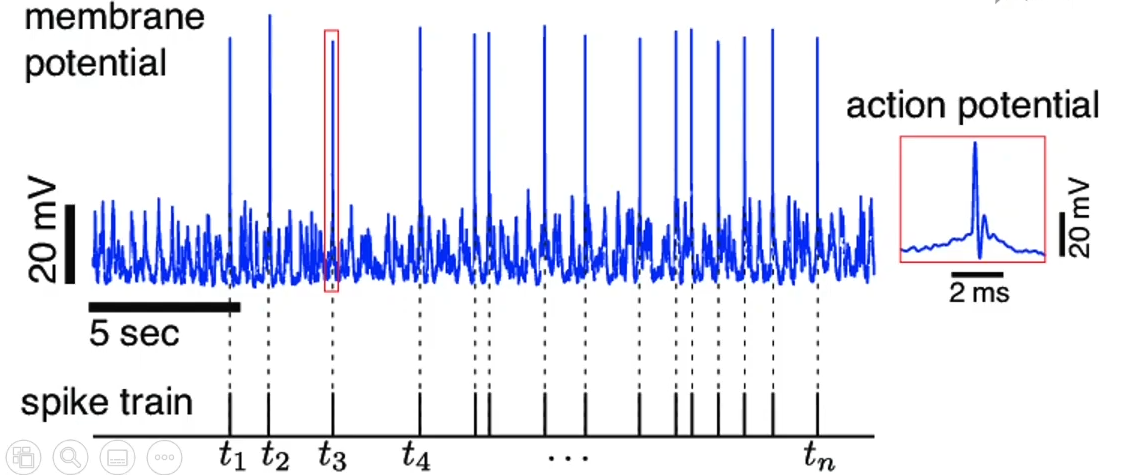
\includegraphics[width=0.7\linewidth]{images/neuronSpikes}
			\caption{Pulsos de um sinal ruidoso. Fonte \cite{dan_goodman_2022_7044500}}
			\label{fig:neuronspike}
		\end{figure}
		
	\subsection{Neurônio de Pulso}
		\par Embora o foco deste trabalho seja nos \textit{Leaky Integrate and Fire Neurons} (LIF) porque são mais simples, mais eficientes e atualmente generalizam melhor para a maioria dos problemas \cite{dan_goodman_2022_7044500}, existem modelos mais biologicamente precisos como o \textbf{neurônio Hodgkin-Huxley} \cite{gerstner2014neuronal} e outros como \cite{jones2020single} que criaram modelos mais próximos aos neurônios naturais explorando a não linearidade dos dendritos e outras características neurais.
		
		\subsubsection{Entendendo o LIF}
			
			\par O LIF é um dos modelos de neurônios mais simples em RNPs, ainda assim, pode ser aplicado com sucesso na maioria dos problemas em que as RNPs podem ser usadas.
			
			\par O LIF, assim como um neurônio de RN, recebe a soma dos inputs ponderados, mas, em vez de passá-lo diretamente para sua função de ativação, algum \textit{vazamento} é aplicado, diminuindo em algum grau a soma.
			
			\par O LIF se comporta muito como circuitos Resistor-Capacitor, como pode ser visto na Figura \ref{fig:rcmodel}. Aqui, $R$ é a resistência ao vazamento da corrente, $I_{in}$ é a corrente de entrada, $C$ é a capacitância, $U_{mem}$ representa é o potencial acumulado e $v$ é um interruptor que permite que o capacitor se descarregue (ou seja, emita um pulso) quando um determinado limiar de potencial é alcançado.
			
			\begin{figure}[H]
				\centering
				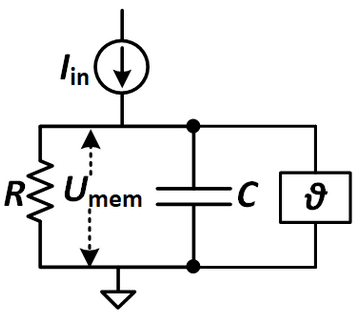
\includegraphics[width=0.4\linewidth]{images/rcmodel}
				\caption[O modelo RC]{Modelo RC: Fonte: \cite{10242251}}
				\label{fig:rcmodel}
			\end{figure}
			
			\par Ao contrário do neurônio Hodgkin-Huxley, os pulsos são representados como \textbf{uns} esparsamente distribuídos em uma sequência de \textbf{zeros}, como ilustrado nas Figuras \ref{fig:pulsossparsitystaticsupress} e \ref{fig:sparsity}. Essa abordagem simplifica os modelos e reduz a potência computacional e o armazenamento necessário para executar uma RNP.
			
			\begin{figure}[H]
				\centering
				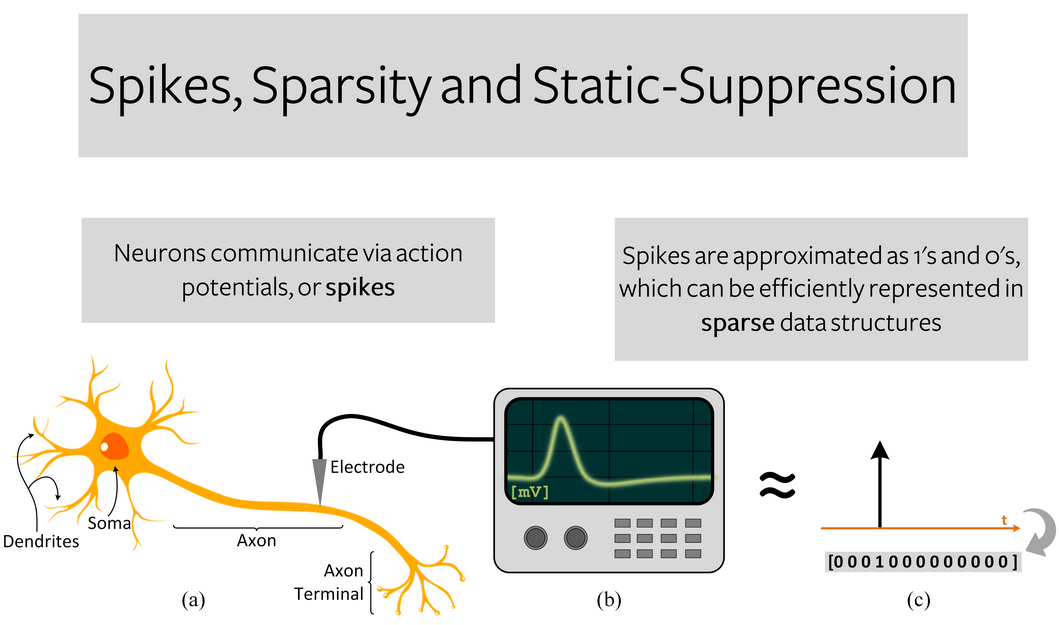
\includegraphics[width=.8\linewidth]{images/spikesSparsityStaticSupress}
				\caption{Esparsidade em Redes Neurais de Pulsos. Fonte: \cite{10242251}}
				\label{fig:pulsossparsitystaticsupress}
			\end{figure}
			
			\begin{figure}[H]
				\centering
				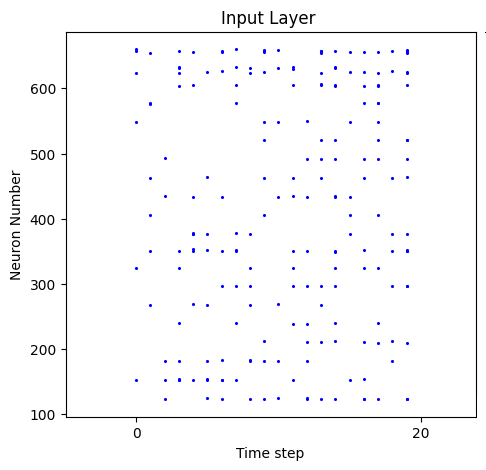
\includegraphics[width=.4\linewidth]{images/sparsity}
				\caption[Atividade esparsa de uma RNP]{Atividade esparsa de uma RNP: O eixo horizontal representa o momento no qual os dados estão sendo processados e o vertical representa o número de neurônios da RNP. Note que, na maior parte do tempo, muito poucos neurônios são ativados. Fonte: O autor.}
				\label{fig:sparsity}
			\end{figure}
						
			\par Como resultado do mencionado acima, em RNP, a informação é codificada no formato de \textit{tempo} e/ou \textit{taxa} de pulsos, proporcionando consequentemente grandes capacidades de processamento de fluxos de dados, mas limitando o processamento de dados estáticos.
			
			\par O modelo LIF é governado pelas equações abaixo \cite{10242251}.
			
			\par Considerando que $Q$ é uma medida de carga elétrica e $V_{\text{mem}}(t)$ é a diferença de potencial na membrana em um determinado tempo $t$, então a capacitância do neurônio $C$ é dada pela Equação \ref{eq:capacitance}.
			
			\begin{equation}
				\label{eq:capacitance}
				C = \frac{Q}{V_{mem}(t)}
			\end{equation}
			
			\par Então, a carga do neurônio pode ser expressa pela Equação \ref{eq:charge}.
			
			\begin{equation}
				\label{eq:charge}
				Q = C.V_{mem}(t)
			\end{equation}
			
			\par To know how these charge changes according to the time (aka current) we can derivate $Q$ as in Equation \ref{eq:rateOfChargeChange}. This expression express the current in the capacitive part of the neuron $I_C$
			
			\par Para saber como essa carga muda ao longo do tempo (ou seja, medir a corrente), podemos derivar $Q$ como na Equação \ref{eq:rateOfChargeChange}. Essa expressão representa a corrente na parte capacitiva do neurônio $I_C$.
			
			\begin{equation}
				\label{eq:rateOfChargeChange}
				I_C = \dfrac{dQ}{dt} = C. \dfrac{dV_{mem}(t)}{dt}
			\end{equation}
			
			\par Para calcular a corrente total passando pela parte resistiva do circuito, podemos usar a lei de Ohm:
			
			\begin{equation}
				\label{eq:ohmlaw}
				V_{mem}(t) = R.I_R \implies I_R = \frac{V_{mem}(t)}{R}
			\end{equation}
			
			\par Então, considerando que a corrente total não muda, como visto na Figura \ref{fig:rcmodel2}, temos a corrente total de entrada $I_{in}$ do neurônio como na Equação \ref{eq:totalNeuronCurrent}.
			
			\begin{figure}[H]
				\centering
				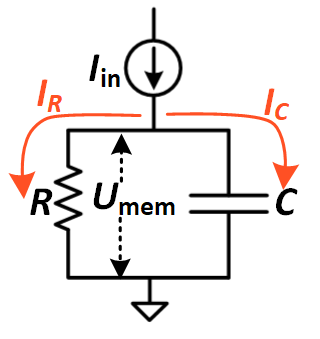
\includegraphics[width=0.3\linewidth]{images/rcmodel2}
				\caption[Modelo RC para correntes]{Modelo RC para correntes: $I_{in} = I_R + I_C$}
				\label{fig:rcmodel2}
			\end{figure}
			
			\begin{equation}
				\label{eq:totalNeuronCurrent}
				I_{in}(t) = I_R + I_C \implies I_{in}(t) = \frac{V_{mem}(t)}{R} + C.\dfrac{dV_{mem}(t)}{dt}
			\end{equation}
		
			\par Portanto, para descrever a membrana passiva, temos a Equação linear \ref{eq:memLinear}.
			
			\begin{equation}
				\label{eq:memLinear}
				\begin{aligned}
					I_{in}(t) &= \frac{V_{mem}(t)}{R} + C.\dfrac{dV_{mem}(t)}{dt} \implies \\ 
					I_{in}(t) - \frac{V_{mem}(t)}{R} &=  C.\dfrac{dV_{mem}(t)}{dt} \implies \\
					\Aboxed{R.I_{in}(t) - V_{mem}(t) &=  R.C.\dfrac{dV_{mem}(t)}{dt}}
				\end{aligned}
			\end{equation}
			
			\par Então, se considerarmos $\tau = R.C$ como a \textbf{constante de tempo da membrana}, obtemos tensões em ambos os lados da Equação \ref{eq:finalMem}, que \textbf{descreve o circuito RC}.
			
			\begin{equation}
				\label{eq:finalMem}
				\begin{aligned}
					R.I_{in}(t) - V_{mem}(t) &=  R.C.\dfrac{dV_{mem}(t)}{dt} \implies \\
					R.I_{in}(t) - V_{mem}(t) &=  \tau.\dfrac{dV_{mem}(t)}{dt} \implies \\
					\Aboxed{\tau.\dfrac{dV_{mem}(t)}{dt} &= R.I_{in}(t) - V_{mem}(t)}
				\end{aligned}
			\end{equation}
			
			\par A partir disso, igualando $I_{in} = 0$ (ou seja, sem entrada) e considerando que $\tau = R.C$ é uma constante e, além disso, atribuindo um potencial inicial $V_{mem}(0)$, o comportamento da voltagem do neurônio pode ser modelado como uma curva exponencial, como visto na Equação \ref{eq:expmembrane}.
			
			\begin{equation}
				\label{eq:expmembrane}
				\begin{aligned}
					\tau.\dfrac{dV_{mem}(t)}{dt} &= R.I_{in}(t) - V_{mem}(t) \implies \\
					\tau.\dfrac{dV_{mem}(t)}{dt} &= -V_{mem}(t) = \\
					e^{\ln(V_{mem}(t))} &= e^{-\frac{t}{\tau}} = \\
					\Aboxed{V_{mem}(t) &= V_{mem}(0).e^{-\frac{t}{\tau}}}
				\end{aligned}
			\end{equation}
			
			\par Então, pode-se dizer que: Na ausência de uma entrada $I_{in}$, o potencial da membrana decai exponencialmente, como ilustrado na Figura \ref{fig:membranepotentialdecay} e implementado no Código \ref{lst:membranepotentialdecay}.
			
			\begin{lstlisting}[language=Python, caption={Python implementation of the action potential decaying of a LIF: $I_{in} = 0$}, label={lst:membranepotentialdecay}]
def lif(V_mem, dt=1, I_in=0, R=5, C=1):
	tau = R*C
	V_mem = V_mem + (dt/tau)*(-V_mem + I_in*R)
	return V_mem
\end{lstlisting}
			
			\begin{figure}[H]
				\centering
				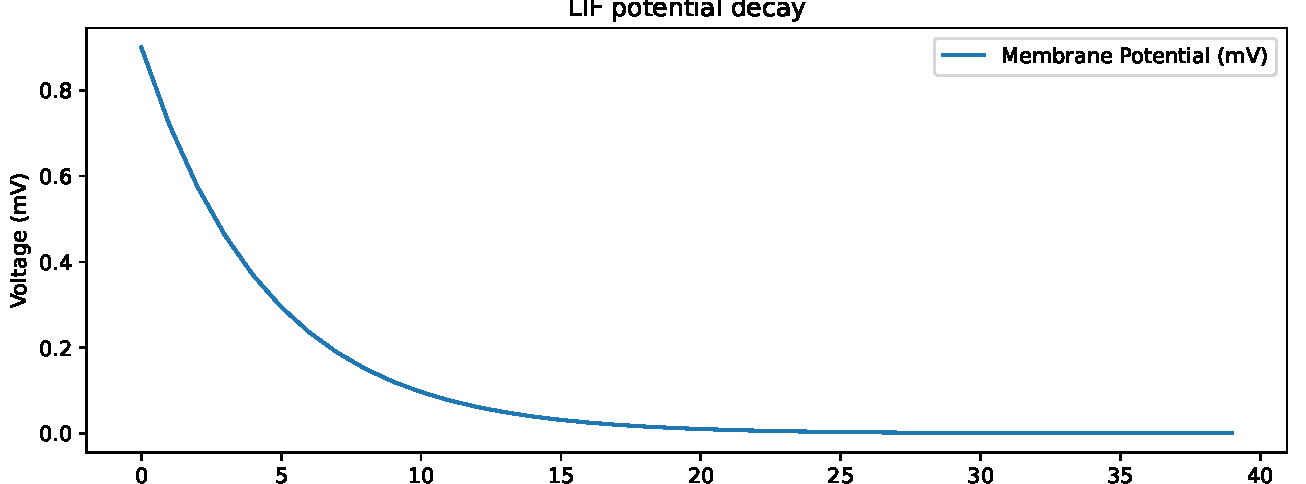
\includegraphics[width=.7\linewidth]{images/membranePotentialDecay}
				\caption{Decaimento do potencial da membrana. Fonte: O autor}
				\label{fig:membranepotentialdecay}
			\end{figure}
			
			\par Com os resultados da Equação \ref{eq:finalMem}, é possível calcular o aumento da voltagem, conforme visto na Equação \ref{eq:actionpotincrease}.
			
			\begin{equation}
				\label{eq:actionpotincrease}
				\begin{aligned}
					&\tau.\dfrac{dV_{mem}(t)}{dt} = R.I_{in}(t) - V_{mem}(t) = \\
					&\dfrac{dV_{mem}(t)}{dt} + \frac{V_{mem}(t)}{\tau} = \frac{R.I_{in}(t)}{\tau} \implies \\
					&\text{Integrating factor: } e^{\int \frac{1}{\tau} dt} = e^{\frac{1}{\tau}.t} \implies \\
					&(e^{\frac{1}{\tau}.t}.V_{mem}(t))' = \frac{R.I_{in}(t)}{\tau}.e^{\frac{1}{\tau}.t} = \\
					&\int (e^{\frac{1}{\tau}.t}.V_{mem}(t))' = \int \frac{R.I_{in}(t)}{\tau}.e^{\frac{1}{\tau}.t} dt = \\
					&e^{\frac{1}{\tau}.t}.V_{mem}(t) = \int \frac{R.I_{in}(t)}{\tau}.e^{\frac{1}{\tau}.t} dt \therefore \\
					& \text{Considering: } V_{mem}(t=0) = 0 \implies \\
					\Aboxed{&V_{mem}(t) = I_{in}(t).R(1-e^{\frac{1}{\tau}})}
				\end{aligned}
			\end{equation}
			
			\par Note que quando os potenciais de ação aumentam, ainda há um comportamento exponencial, como visto na Figura \ref{fig:membranepotentialincrease} e implementado no Código \ref{lst:membranepotentialincrease}.
			
			\begin{lstlisting}[language=Python, caption={Python implementation of the action potential decreasing of a LIF: $I_{in}=1$}, label={lst:membranepotentialincrease}]
	
def lif(V_mem, dt=1, I_in=1, R=5, C=1):
	tau = R*C
	V_mem = V_mem + (dt/tau)*(-V_mem + I_in*R)
	return V_mem
\end{lstlisting}
			
			\begin{figure}[H]
				\centering
				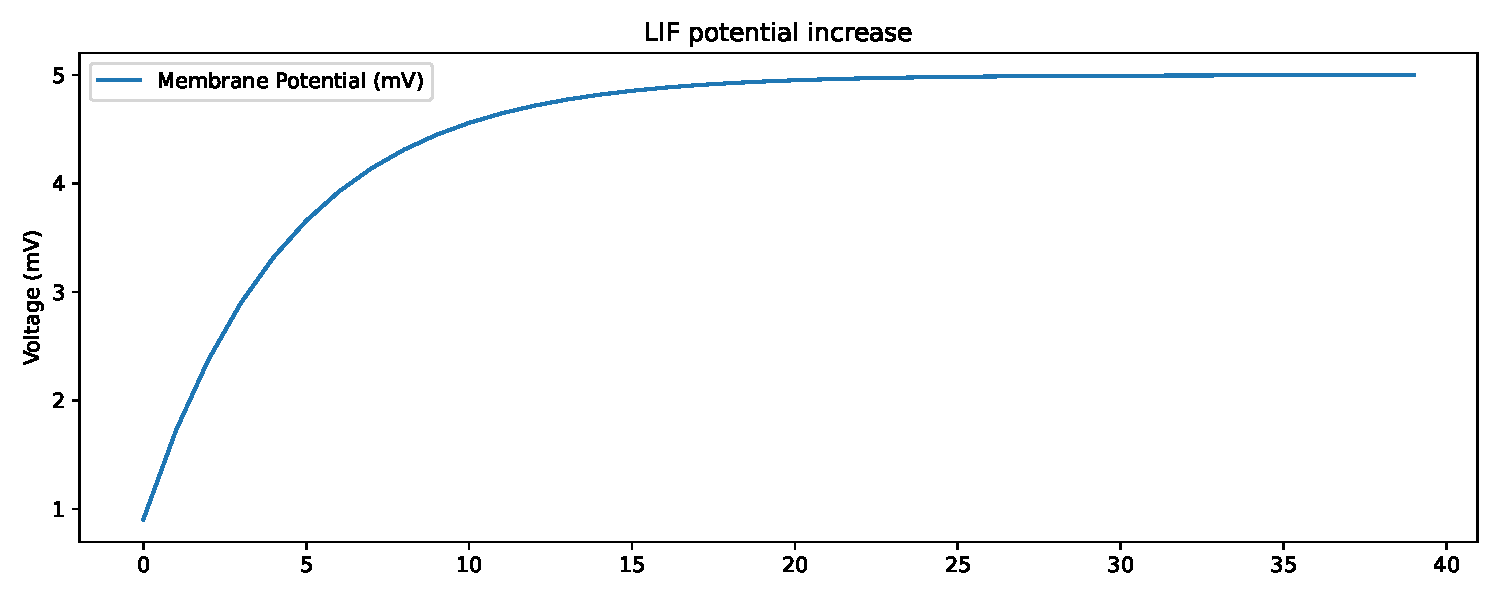
\includegraphics[width=.7\linewidth]{images/membranePotentialIncrease}
				\caption{Aumento do potencial da membrana. Fonte: O autor}
				\label{fig:membranepotentialincrease}
			\end{figure}
			
			\par Levando em consideração um certo \textbf{limiar} que indica um \textit{reset} nvoltagem do neurônio e dois tipos de \textit{resets} (para zero e subtração do limiar), finalmente é possível modelar o comportamento completo do LIF, conforme ilustrado na Figura \ref{fig:membranepotentialfull} e implementado no Código \ref{lst:membranepotentialfull}:
			
			\begin{lstlisting}[language=Python, caption={Python implementation of the action potential full simulation of a LIF: $I_{in}=1$, $V_{thresh} = 2$ is threshold}, label={lst:membranepotentialfull}]
def lif(V_mem, dt=1, I_in=1, R=5, C=1, V_thresh = 2, reset_zero = True):
	tau = R*C
	V_mem = V_mem + (dt/tau)*(-V_mem + I_in*R)
	if V_mem > V_thresh:
		if reset_zero:
			V_mem = 0
		else:
			V_mem = V_mem - V_thresh
	return V_mem
\end{lstlisting}

			
			\begin{figure}[H]
				\centering
				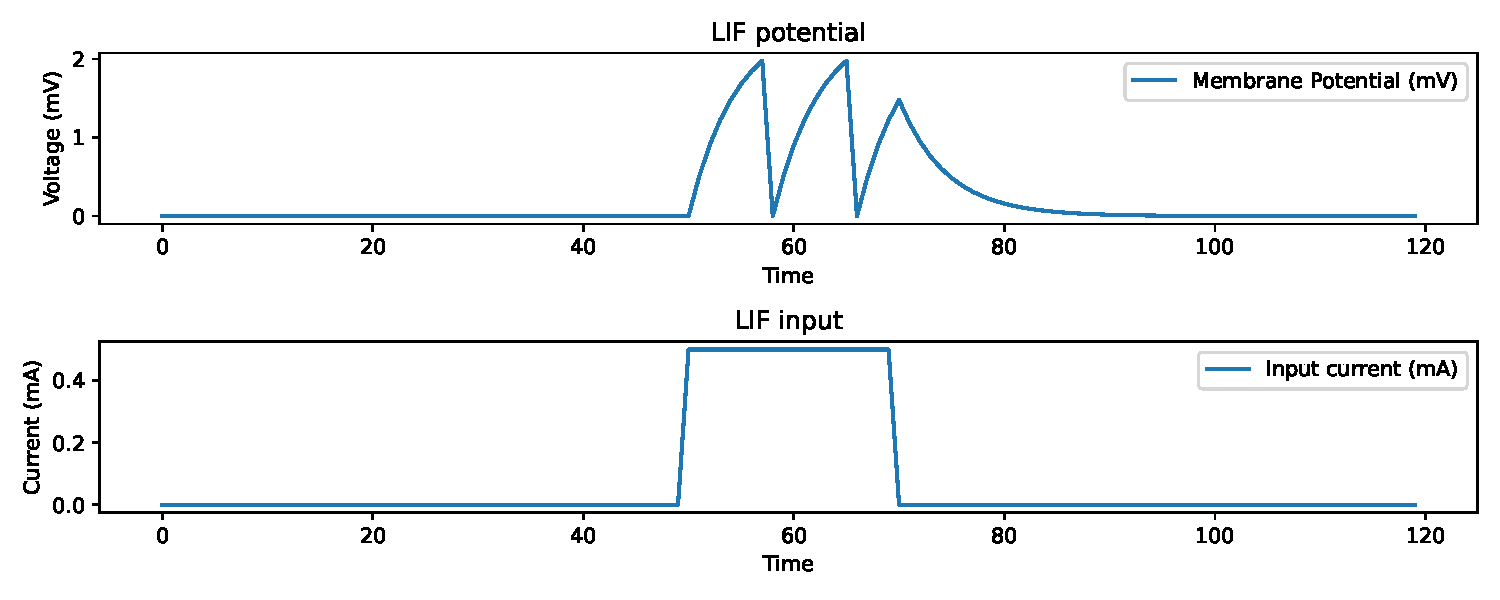
\includegraphics[width=.8\linewidth]{images/membranePotentialFull}
				\caption{Gráfico do LIF simulado completo: Foram fornecidos 0.5 mA de corrente no intervalo de tempo de 51 a 70. Fonte: O autor}
				\label{fig:membranepotentialfull}
			\end{figure}

			
		\subsection{Outra interpretação do LIF}
			
			\par Começando com a Equação \ref{eq:finalMem} e usando o Método de Euler para resolver o modelo LIF:
			
			\begin{equation}
				\tau.\dfrac{dV_{\text{mem}}(t)}{dt} = R.I_{\text{in}}(t) - V_{\text{mem}}(t)
			\end{equation}
			
			\par Resolvendo a derivada na Equação \ref{eq:membraneDerivative}, obtemos o potencial da membrana para qualquer tempo $t+\Delta t$ no futuro:
			
			\begin{equation}
				\label{eq:membraneDerivative}
				\begin{aligned}
					\tau.\dfrac{V_{\text{mem}}(t+\Delta t) - V_{\text{mem}}(t)}{\Delta t} &= R.I_{\text{in}}(t) - V_{\text{mem}}(t) = \\
					V_{\text{mem}}(t+\Delta t) - V_{\text{mem}}(t) &= \frac{\Delta t}{\tau} . (R.I_{\text{in}}(t) - V_{\text{mem}}(t)) = \\
					\Aboxed{V_{\text{mem}}(t+\Delta t) &= V_{\text{mem}}(t) + \frac{\Delta t}{\tau} . (R.I_{\text{in}}(t) - V_{\text{mem}}(t))}
				\end{aligned}
			\end{equation}

		\subsection{Treinamento}
		
			\par \textbf{Como as RNPs são treinadas?} Bem, esta ainda é uma questão em aberto. Um neurônio RNP tem o comportamento de sua função de ativação mais parecido com uma \textbf{função de passo}. Portanto, em princípio, não podemos usar soluções baseadas em descida de gradiente porque esse tipo de função \textbf{não é} diferenciável \cite{kasabov2019time}.
			
			\par Mas existem algumas ideias que podem lançar alguma luz sobre este assunto: Enquanto algumas observações \textit{in vivo/in vitro} mostram que os cérebros, em geral, aprendem fortalecendo/enfraquecendo e adicionando/removendo sinapses ou até mesmo criando novos neurônios ou outros métodos complicados como pacotes de RNA, existem algumas mais aceitáveis como as da lista abaixo \cite{kasabov2019time}:
			
			\begin{itemize}
				\item \textbf{Plasticidade Dependente do Tempo de Pulsos (STDP)}: Se um neurônio pré-sináptico dispara \textbf{antes} do pós-sináptico, há um fortalecimento na conexão, mas se o neurônio pós-sináptico disparar antes, então há um enfraquecimento.
				\item \textbf{Descida de Gradiente Emprestada}: Aproxima a função de passo usando outra função matemática, que é diferenciável (como uma sigmoide), para treinar a rede. Essas aproximações são usadas apenas na fase de \textit{backpropagation}, enquanto mantêm a função de passo na fase do \textit{feed-forward} \cite{kasabov2019time}.
				\item \textbf{Algoritmos Evolutivos}: Usam a seleção dos mais aptos ao longo de muitas gerações de redes.
				\item \textbf{Reservatório/Computação Dinâmica}: \textbf{Redes de estado de eco} ou \textbf{Máquinas de estado líquido}, respectivamente.
			\end{itemize}
		
		\subsection{Autoencoders}
		
			\par Como ilustrado na Figura \ref{fig:autoencoder} \textit{Autoencoders} são redes neurais treinadas para reconstruir seus dados de entrada. Elas consistem em uma função codificadora, denotada como $h = f(x)$, e uma função decodificadora que produz uma reconstrução, denotada como $r = g(h)$. A camada oculta $h$ representa um \textbf{código} ou representação comprimida da entrada \cite{Goodfellow-et-al-2016}. \newline
			
			\par O principal objetivo de um \textit{autoencoder} é aprender uma representação dos dados de entrada na camada de código e, em seguida, reconstruir os dados de entrada com a maior precisão possível usando o decodificador. Geralmente, os \textit{autoencoders} são projetados para serem incapazes de copiar perfeitamente os dados de entrada. Eles tem sua camada de código limitada em dimensionalidade para apenas aproximar a entrada e priorizar certos aspectos dos dados extraindo dessa forma os componentes mais cruciais e significativos de uma dada entrada, o nome dado a esses \textit{autoencoders} é \textbf{Autoencoders subcompletos} \cite{Goodfellow-et-al-2016}.\newline
			
			\par \textit{Autoencoders} podem ser treinados usando várias técnicas, como \textit{gradient descent} com \textit{minibatch} ou estocástico \cite{Goodfellow-et-al-2016}.
	
			\begin{figure}[H]
				\centering
				\caption[autoencoder]{\textit{Autoencoder}: $x$ é codificado para uma dimensão menor $h$ e, em seguida, é reconstruído em $r$, tal processo pode implicar ou não em uma perda na reconstrução}
				\begin{tikzpicture}[node distance=1.5cm, every edge/.style={draw=black,->}]
	% Nodes
	\node[draw, circle] (x) {$x$};
	\node[draw, rectangle, above right=0.7cm and 1cm of x] (encoder) {Codificador};
	\node[draw, circle, above right=0.7cm and 1cm of encoder] (h) {$h$};
	\node[draw, rectangle, below right=0.7cm and 1cm of h] (decoder) {Decodificador};
	\node[draw, circle, below right=0.7cm and 1cm of decoder] (r) {$r$};
	
	% Arrows
	\draw (x) edge (encoder);
	\draw (encoder) edge (h);
	\draw (h) edge (decoder);
	\draw (decoder) edge (r);
	
	% Loss
	\node[below of=h, yshift=-0.7cm] (loss) {Perda na reconstrução};
	\draw (x) edge (loss);
	\draw (r) edge (loss);
	
	% Labels
	\node[below of=x, yshift=0.7cm] {Entrada};
	\node[below right=0.2cm and 0.8cm of decoder] {Saída};
	\node[below of=r, yshift=0.7cm] {Entrada reconstruida};
\end{tikzpicture}
				\label{fig:autoencoder}
			\end{figure}
			
			\par Considerando-se que a reconstrução $r$ seja razoável, isso significa que a região $h$  contém dados suficientes para representar a informação em sua essência, sendo assim, dentro do contexto das redes neurais, \textit{autoencoders} são ótimos produtores de vetores de características. Hipoteticamente é possível criar \textit{autoencoders} cuja a camada de código seja apenas um número inteiro caso tanto o codificador quanto o decodificador sejam grandes e complexos o suficiente mas isso se mostraria inútil caso se necessitasse algum tipo de representação da informação original que fosse significativa, ademais, excluindo-se casos triviais, segundo \citeauthor{Goodfellow-et-al-2016} isso ainda não se verificou na prática.
	
		\subsection{Redes neurais residuais (ResNets)}
			\par Segundo \cite{DBLP:journals/corr/HeZRS15} a ideia-chave por trás do \textit{ResNets} é a inclusão de conexões de salto como ilustrado na Figura \ref{fig:residualblock}, também conhecidas como mapeamentos de identidade, que permitem que a saída de uma camada seja adicionada diretamente à entrada da camada subsequente. Isso contorna as camadas intermediárias e garante que redes mais profundas possam aprender. Outra vantagem no uso de conexões de salto é que essa prática diminui a ocorrência de \textit{vanishing gradients} um problema comum em redes com muitas camadas que pode impossibilitar ou diminuir a níveis impraticáveis o aprendizado da rede.
			
			\begin{figure}
				\centering
				\caption[bloco de uma Resnet]{Bloco de uma Rede Neural Residual, $X$ é uma função identidade que contorna as camada intermediárias criando "\textit{highway connections}"}
				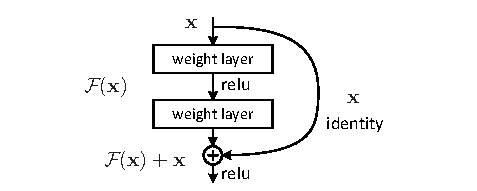
\includegraphics[width=0.7\linewidth]{images/residualBlock}
				\\ Fonte: \cite{DBLP:journals/corr/HeZRS15}
				\label{fig:residualblock}
			\end{figure}